
%%
%% This document created by A.Tasora
%%

\documentclass[review]{elsarticle}

%%
%% Additional packages... --------------------------------------------------
%%


\usepackage{graphicx}
\usepackage{epstopdf}
\usepackage{amsmath, amssymb}
\usepackage{amssymb}
\usepackage{psfrag}
\usepackage{siunitx}
\usepackage{booktabs}
%\usepackage[english]{alg}
\usepackage{algpseudocode}
% \usepackage{authblk}
\usepackage{subcaption}
\usepackage{hyperref}
% \usepackage{bm}
% \include{BibFEM.bib}

\sloppy

%% A.TASORA CUSTOM TEX COMMANDS:
%%
 
\def\avect#1{{\boldsymbol{#1}}}
\def\amatr#1{{\boldsymbol{#1}}}




%%%%%%%%%%%%%%%%%%%%%%%%%%%%%%%%%%%%%%%%%%%%%%%%%%%%%%%%%%%%%%%%%%%%%%%%%%%%%%%%%%%%
%%%%%%%%%%%%%%%%%%%%%%%%%%%%%%%%%%%%%%%%%%%%%%%%%%%%%%%%%%%%%%%%%%%%%%%%%%%%%%%%%%%%




\begin{document}


%%
%% TITLE
%%


\title{A geometrically exact isogeometric beam for large displacements and contacts}

%\author{Alessandro Tasora \\ alessandro.tasora@unipr.it}
\author{Alessandro Tasora}
\ead{alessandro.tasora@unipr.it}
\author{Simone Benatti}
\ead{simone.benatti@studenti.unipr.it}
\author{Dario Mangoni}
\ead{dario.mangoni@unipr.it}
\author{Rinaldo Garziera}
\ead{rinaldo.garziera@unipr.it}
\address{Universit\`a degli Studi di Parma, \\Dpt. of Engineering and Architecture\\Parco Area delle Scienze, 181/A, 43124 Parma, Italy }

% \affil[]{Universit\`a degli Studi di Parma, \\ 
% Dpt. of Engineering and Architecture, Parco Area delle Scienze, 181/A, 43124 Parma, Italy 
% \footnote{E-mail addresses: alessandro.tasora@unipr.it (A. Tasora), \\ simone.benatti@studenti.unipr.it (S. Benatti) dario.mangoni@studenti.unipr.it (D. Mangoni), rinaldo.garziera@unipr.it (R.Garziera).}
% }


% \newcommand{\avect}[1]{{\boldsymbol{#1}}}
% \newcommand{\amatr}[1]{{\boldsymbol{#1}}}


%\thispagestyle{fancy}

\begin{abstract} 
This work discusses an efficient formulation of a geometrically exact three-dimensional beam which can be used in dynamical simulations involving large displacements, collisions and non-linear materials. To this end, we base our model on the shear-flexible Cosserat rod theory and we implement it in the context of Isogeometric Analysis (IGA). 
According to the IGA approach, the centerline of the beam is parameterized using splines; in our work the rotation of the section is parameterized by a spline interpolation of quaternions, and time integration of rotations is performed using the exponential map of quaternions. Aiming at an efficient and robust simulation of contacts, we propose the adoption of a non-smooth dynamics formulation based on differential-variational inequalities. 
The model has been implemented in an open-source physics simulation library that can simulate actuators, finite elements, rigid bodies, constraints, collisions and frictional contacts. 
This beam model has been tested on various benchmarks in order to assess its validity in non-linear static and dynamic analysis; in all cases the model behaved consistently with theoretical results and experimental data. 
\end{abstract}

\begin{keyword}
IGA \sep beam \sep contact \sep multibody \sep non-smooth dynamics
\end{keyword}

\maketitle

%%

%% SECTIONS
%%


\section{Introduction}

Deformable three-dimensional beams withstanding large displacements can be found in many scenarios of practical interest, this is the case of the blades in a helicopter rotor, for instance, or the case of the torsion bar in a car suspension, or the case of a flexible robot arm. In the last decades, similar problems motivated extensive research in the area of fast, robust and reliable computer methods for the simulation of beams, and most of those methods are based on Finite Element (FE) discretizations.

Recently, the Isogeometric Analysis (IGA) computational approach gained increased popularity as it blends the concept of spline interpolation in the context of FE. 
While traditional FE methods discretize the continuum using finite elements that share end nodes, the IGA approach uses a single spline with several nodes. Indeed, nowadays most CAD tools are based on splines of NURBS or B-spline type, hence one of the relevant advantages of IGA is that these geometries can be imported directly in the simulation, whereas FE methods require an intermediate pre-processing step in order to generate a mesh approximation of the original geometry~\cite{HUGHES2005}. Moreover, conventional finite elements using Lagrange polynomials feature $C^0$ continuity at nodal points regardless of their order, while spline functions of order $p$ provide $C^{p-1}$ continuity at all non-multiple knots. This  means that for the same amount of degrees of freedom, IGA shows better robustness and accuracy compared to $C^0$-continuous FE~\cite{COTTRELL2007refinement}.

Although the most obvious application of IGA is in the modeling of structural elements which can map to a line parameterization, such as cables and beams, the same concept can be extended to generic PDEs involving membranes, shells and volumes~\cite{COTTRELL20065257,Benson2010IGAShells}.
Among the vast literature on IGA, we cite in passing the developments on hierarchical refinement~\cite{VUONGSIMEON2011hierarchical}, the generalization to T-splines~\cite{BAZILEVS2010tsplines}, the application to fluid dynamics~\cite{Bazilevs2008fluid} and to contact problems~\cite{Wriggers2012mortar,TEMIZER2014interiorpoint}.

In this paper we use IGA to implement a geometrically exact three-dimensional beam based on the Cosserat rod theory, hence capable of arbitrary large rotations and displacements~\cite{LINN2011cosserat}. Non-linear geometric effects in beams have been studied extensively in computational mechanics and different approaches have been put forward: for example a straightforward method still used nowadays is based on reusing linear finite elements developed for infinitesimal-strain conventional beams of Euler-Bernoulli or Timoshenko type, by updating a local corotational reference frame that can have large displacements and rotations~\cite{Crisfield1990corotational,Felippa2005unified}. In contrast to this, but at the cost of a more sophisticated formulation, the \textit{geometrically exact beam model}, also referred to as Simo-Reissner beam model, draws on the theory of 1D Cosserat continua \cite{cosserat1909} and leads to a general formulation that makes no assumption on the amount of rotations and that allows finite strains, including shear and torsion~\cite{Reissner1973gebt,Antman1974,Simo1985finitestrain}.
%Although some beam theories that consider out-of-plane and in-plane deformations of the cross-sections, we will make the assumption of rigid sections.
The Cosserat rod theory does not require that cross-sections must be orthogonal to the tangent of the centerline, hence it can account for shear effects similarly to the Timoshenko beam theory, of whom it can be considered a generalization to the 3D case~\cite{Timoshenko1921Beams}. In fact, Reissner, Kirchhoff-Love, Timoshenko and Euler-Bernoulli beams can be interpreted as special cases of Cosserat rods. 

Many references on IGA-based beams can be found in literature: for instance IGA for Kirchhoff-Love and Euler-Bernoulli beams are discussed in~\cite{GRECO2013kirchhoffbeams} and~\cite{Weeger2013euler}, straight and curved 2D Timoshenko beams are discussed in~\cite{BOUCLIER2012thick}, to name a few. Similarly to FE beams, numerical locking artifacts can affect IGA beams when shear is taken into account. In this context, a collocation approach was used in~\cite{Beiraodaveiga2012IGA,Auricchio2013IGA} to obtain a locking-free spatial IGA beam. 

Contact between three-dimensional rods has been dealt in literature by various authors. Among the first results, in \cite{wriggers1997} a frictionless point-wise contact  formulation was developed between pairs of cables with circular section, later extended to the frictional case \cite{wriggers2000}. The problem of contact between beams of rectangular section, that might generate multiple contact points between the edges, has been discussed in \cite{Wriggers2002,litewka2002frictional}. The issue of self-contact between beams has been studied in \cite{chamekh2009,GayNeto2015}, a topic of great importance if one needs to simulate problems such as the tightening of knots, knitting machines or winches.
Most contact models in literature are based on point-based formulations where the position of contact points is obtained by solving local sub-problems of distance minimization between curved geometries \cite{konyukhov2010}. However this approach is near singular when beams intersect with small contact angles: in \cite{meier2016,meier2017} an efficient method has been proposed that can solve this issue.
In \cite{weeger2018frictional} the simulation of frictional contact and self collision is discussed for a class of efficient IGA-based Cosserat rods.

Similarly to~\cite{Weeger2017IGA}, we address the case of a three-dimensional Cosserat rod of high generality, hence accounting for shear, torsion, geometric and material non-linearity. As an alternative to penalty-based beam contact formulations as presented in~\cite{Weeger2017361}, we express it with a formalism that fits well in a time stepper for non-smooth multibody dynamics, using the theory of Differential Variational Inequality (DVI). 
To our knowledge, this is the first time an IGA formulation has been used in the framework of DVI non-smooth dynamics; the benefit being the fact that DVI formulations provide a robust and stable way to simulate contact problems even with large time-steps and many simultaneous contacts.
 
Early work on non-smooth dynamics can be traced back to the seminal research of Jean-Jacques Moreau on measure-differential inclusions, a special type of DVI \cite{moreau88,Moreau1987}. The non-smooth nature of dynamical problems originates from various phenomena, most often it is a consequence of the Coulomb friction model and impulsive collisions at contact points; instead than regularizing the contact forces -a conventional method that leads to smooth but stiff differential problems- Moreau proposed to embed such set-valued force laws directly in the formulation. This can be done at the cost of assuming that velocities can be discontinuous, hence accelerations are considered as distributions of vector signed measures. Since then, different authors contributed to the field of non-smooth dynamics, see for example \cite{stew98,AniHa02,pfeiffer}. 
The robustness and stability of DVI methods motivated their use in scenarios that involve millions of simultaneous contacts, such as granular dynamics \cite{NegTasLeveraging2011}, or in contexts that require real-time performance and large time steps, such as robotics and virtual reality \cite{bender2014interactive}. Most time stepping schemes for DVI require the solution of a variational inequality (VI) per each time step: early approaches were based on fixed point iterations that both represented a major computational bottleneck and performed badly in presence of finite elements, but recent researches address both issues and stimulate novel applications of DVI methods also to flexible structures \cite{Mazhar2015,heyn2013,MANGONI2018351}. 


In order to test our geometrically-exact rod formulation, we implemented it using the C++ language and we embedded it in our CHRONO open source simulation library~\cite{chrono2013}. We used this library to simulate IGA beams in a broader context involving rigid body dynamics, finite elements, motors, actuators and non-smooth frictional contacts: tests presented at the end of the paper show that the geometrically-exact IGA beam represents an efficient, compact and general way to simulate complex problems involving deformable beams.


% citare: 
%~\cite{Auricchio2013IGA} (Locking-free isogeometric collocation methods for spatial Timoshenko rods) CITATO
%~\cite{Weeger2017IGA} (Isogeometric collocation methods for Cosserat rods) CITATO
%~\cite{Timoshenko1921Beams} CITATO
%~\cite{Wriggers2012mortar} (large deformation contact w.mortar and augmented Lagrangian) CITATO
%~\cite{TEMIZER2014interiorpoint} (interior point method for IGA contact} CITATO
%\cite{LINN2011cosserat} (Cosserat rod) CITATO
%\cite{Lang2011CosseractRods} (Cosserat rot, quaternions) CITATO
%\cite{Reissner1973gebt} (large displacement curved beams, GEBT) CITATO
%\cite{Antman1974} (kirchoff, GEBT) CITATO
%\cite{SIMO1985} (GEBT) CITATO
%\cite{GRECO2013kirchhoffbeams} (IGA kirchoff-love beams} CITATO
%\cite{Weeger2013euler} (IGA Euler-bernoulli) CITATO





\section{B-Splines and NURBS}

Since our beam model draws on Basis splines (B-Splines) or Non-Uniform Rational B-Splines (NURBS), basic concepts about these functions are introduced here.

\subsection{B-Splines}

A B-Spline of order \emph{p} is a piecewise polynomial function of degree \emph{p-1} in a parametric variable $\tau \in \mathbb{R}$ (a curvilinear abscissa).

We introduce a set of $n+1$ control points $\avect{x}_i \in \mathbb{R}^3 \quad i = 0...n$ and a set \emph{n+p+1} of non-decreasing breaking points defining a \emph{knot vector} $\avect{T} =(\tau_0, \tau_1... \tau_{n+p})$. 

\paragraph{Basis Functions} $N_{i,p}$ is an order \emph{p} and \emph{p-1} degree \emph{Basis Function} on the \emph{i-th} knot of the B-Spline and it is recursively defined as follows:
\begin{equation}
\label{eq:BSplineBasis_start}
N_{i,1}(\tau) =\begin{cases}
    1 & \text{for}\qquad \tau_i \leq \tau \leq\ \tau_{i+1}\\
    0 & \text{otherwise}
\end{cases}
\end{equation}
And, for $p>1$:
\begin{equation}
\label{eq:BSplineBasis_iter}
N_{i,p}(\tau) = \frac{\tau-\tau_i}{\tau_{i+p-1}-\tau_i}N_{i,p-1}(\tau) + \frac{\tau_{i+p}-\tau}  {\tau_{i+p}-\tau_{i+1}}N_{i+1,p-1}(\tau) 
\end{equation}
Basis Function are a partition of unity: it means that $\sum_{i=0}^nN_{i,p}(\tau)=1 \quad \forall \tau \in [\tau_o, \tau_n]$. 
The span of Basis Function increases with the order \emph{p}. \newline
Is useful to remind the derivative of the Basis Function with respect to the parametric variable since it is frequently used:
\begin{equation}
\label{BSplineBasis_derivative}
\mathring{N}_{i,p}(\tau) = \frac{dN_{i,p}(\tau)}{d\tau} = \frac{p-1}{\tau_{i+p-1}-\tau_i}N_{i,p-1}(\tau) - \frac{p-1}{\tau_{i+p}-\tau_{i+1}}N_{i+1,p-1}(\tau) 
\end{equation}
\paragraph{B-Splines formulation} A B-Spline is a linear combination of control points $\avect{x}_i$ and Basis Functions $N_{i,p}(\tau)$
\begin{equation}
\label{eq:BSpline}
\avect{r}(\tau) = \sum_{i=0}^n \avect{x}_i N_{i,p}(\tau) \qquad\qquad n \geq p-1
\end{equation}
Given the number of control points \emph{n+1} and the order of the curve $p$ the number of knots is $n+p+1$, which means there are more knots than control points, so some knots can be coincident on the same control point. When knots are distinct the first $p-1$ derivatives are continuous; when $r$ nodes are coincident, only the first $p-r$ derivatives are continuous. In general, control points do not lie on the curve. When $p$ knots are coincident, the spline passes through the control point with $C^0$ continuity.


\subsection{NURBS}

Non-Uniform Rational B-Splines introduce additional weights ${w_i}>0$, $(i = 1...n)$, so that \emph{rational} basis $R_{i,p}(\tau)$ are used in place of $N_{i,p}(\tau)$:
\begin{equation}
\label{eq:NURBS_Basis}
R_{i,p}(\tau) = \frac{N_{i,p}(\tau)w_i}{\sum_{j=1}^n N_{j,p}(\tau)w_j}
\end{equation}
NURBS have the same properties listed for B-Splines: in particular for $w_i = 1 \; \forall i$, NURBS reduce to B-Splines. In addition, by using proper weights and few coarse control points, NURBS allow the exact (not approximated) representation of conic sections like circles and ellipses; this is a relevant feature because canonical primitives in CAD models are most often built from conical sections.


% THE SECTION ON ROTATIONS AND LIE GROUPS HAS BEEN 
% REMOVED.
% JUST REMOVE THE COMMENT BEFORE \input{} TO GET IT BACK.
%
%\input{"chapter_rotations.tex"}




\section{Kinematics of Cosserat rods}

Our implementation of IGA beams draws on the Cosserat rod theory.
This implies that the rotation of the beam section is independent 
from the centerline position. This differs from the Euler-Bernoulli or
Kirchhoff beam theory which implies that sections remain orthogonal to the centerline,
an assumption that holds only for thin beams, because shear effects
cannot be modelled. 
%On the other hand the Timoshenko theory, at the cost of introducing rotational degrees of freedom per each node, allows also to model shear effects in thick beams. 


\subsection{Configuration}

A Cosserat beam is represented by the line of its mass centroids (\emph{centerline}), which is described by a curve parameterized~\cite{Weeger2017IGA} by a curvilinear abscissa $s \in [0,T] $:
%
\begin{equation}
	\avect{r} = \avect{r}(s) \quad \in \mathbb{R}^3
\end{equation}

Section rotations $\amatr{R}$ are parameterized by  the same curvilinear abscissa $s \in [0,T] $ (even though not mandatory~\cite{Auricchio2013IGA} ), assuming that the $X$ axis of the $\amatr{R}$ frame represents the normal of the beam section, and $Y$ and $Z$ 
axes represent the height and width directions, respectively:
%
\begin{equation}
	\amatr{R} = \amatr{R}(s) \quad \in \mathsf{SO}(3)
\end{equation}

That is, at some point $s_a$ along the curve we have independent positions and rotations: 
$\avect{r}(s_a)$, $\amatr{R}(s_a)$.

We remark a first source of complication: $\amatr{R}$ is a 3D rotation matrix, that is a 3x3 orthogonal matrix (hence
the \emph{special orthogonal group} $\mathsf{SO}(3)$ in the terminology of Lie groups). Its 3x3 elements are not independent as $\amatr{R}\amatr{R}^T=\amatr{I}$ must hold: in general it is better to avoid using all nine elements of such matrix and use quaternions or rotation angles to parameterize rotation frames~\cite{Lang2011CosseractRods}. 


\subsection{Strains}

Following~\cite{Simo1986finitestrain}, we can express  
$\underline{\avect{\epsilon}}$ and $\underline{\avect{\kappa}}$, hereafter called translational strains and rotational strains, respectively. 
% Simo86 Table 2
The translational strain $\underline{\avect{\epsilon}}$ is:
%
\begin{equation}
	\underline{\avect{\epsilon}} = \amatr{R}^T \avect{r}' - \avect{e_x}
	\label{eq:epsilon}
\end{equation}
%
where we introduced $\avect{e_x} = \{1,0,0\}$ and we introduced the \emph{curve gradient} 
%
\begin{equation}
\avect{r}' = \frac{d\avect{r}}{ds}. 
\end{equation}

Note that for an
undeformed beam we have $\amatr{R}^T\avect{r}' = \{1,0,0\}$, that is we assume that $s$ 
is a uniform arc-length parameterization. Is other words, at the initial state,
the curvilinear length of a curve from $s=a$ to $s=b$, i.e. $L=\int^b_a ||\avect{r}'||ds$, is exactly $b-a$. Usually, 
however, splines are not parameterized with uniform arc-length abscissa, because a 
generic abscissa $\tau$ is used instead. If so, we have  
%
\begin{equation}
\avect{r}' = \frac{d\avect{r}}{d\tau} \frac{d\tau}{ds} = \mathring{\avect{r}} J^{-1}
\end{equation}
%
where a jacobian is defined as $J_{s\tau} = \frac{ds}{d\tau}$, and $\mathring{\avect{r}} =\frac{d\avect{r}}{d\tau}$ is the parametric derivative (something that is quite easy to compute when dealing with splines).

During an initialization phase, when the beam is still undeformed, values of jacobians $J_{s\tau}$ are computed and stored in memory for all the integration points - they will be used later, when computing the internal forces.

The rotational strain  $\underline{\avect{\kappa}}$ is computed as~\cite{Weeger2017IGA}:
%
\begin{equation}
	\tilde{\underline{\avect{\kappa}}} = \amatr{R}^T \amatr{R}'
\end{equation}
%
Here $\amatr{R}' = \frac{d\amatr{R}}{ds}$ , while the tilde operator means:
%
\begin{equation}
	\tilde{\underline{\avect{\kappa}}} = 
	\left[  
	\begin{array}{ccc}
	 0 & -\kappa_z & \kappa_y \\
	 \kappa_z & 0 & -\kappa_x \\
	 -\kappa_y & \kappa_x & 0 
	\end{array}
	\right]
\end{equation}
%
so it is obvious that one can build $\underline{\avect{\kappa}}$ from $\tilde{\underline{\avect{\kappa}}}$ or vice versa.

Finally, in case the beam starts in an initially-curved configuration, initial values $\underline{\avect{\epsilon}}_0$ and $\underline{\avect{\kappa}}_0$ can be computed using the expression above, then one would compute effective strains with:
%
\begin{align}
	\avect{\epsilon} &= \underline{\avect{\epsilon}} - \underline{\avect{\epsilon}}_0 \\
	\avect{\kappa}   &= \underline{\avect{\kappa}} - \underline{\avect{\kappa}}_0 
\end{align}



\subsection{Constitutive model}

Once $\avect{\epsilon}$ and $\avect{\kappa}$ are computed, with some generic constitutive model one can compute their conjugate vectors, i.e. the generalized cut-section forces $\avect{n}$ and cut-section torques $\avect{m}$, henceforth called translational stresses and rotational stresses, respectively.
The most generic constitutive model is expressed by a non-linear function:
%
\begin{align}
  \left\{  
	 \avect{\epsilon},
	 \avect{\kappa}
	\right\} \in \mathbb{R}^6
	\rightarrow
	\left\{  
	 \avect{n},
	 \avect{m} 
	\right\} \in \mathbb{R}^6
\label{eq:mnconstitutive}
\end{align}

Note that $\avect{n}$ and $\avect{m}$ are expressed in the local coordinate system of the section frame: if one
needs the absolute values of such vectors, they can be computed easily, later, as 
% Simo 86 eq 2.3
\begin{align}
\avect{n}_a &= \amatr{R}\avect{n}\\ 
\avect{m}_a &= \amatr{R}\avect{m}
\end{align}

When structural damping is needed, instead of \eqref{eq:mnconstitutive} we use:
%
\begin{align}
  \left\{  
	 \avect{\epsilon},
	 \avect{\kappa},
	 \dot{\avect{\epsilon}},
	 \dot{\avect{\kappa}}
	\right\} \in \mathbb{R}^{12}
	\rightarrow
	\left\{  
	 \avect{n},
	 \avect{m} 
	\right\} \in \mathbb{R}^6
\label{eq:mnconstitutivewdamping}
\end{align}
%
by introducing the %
 strain derivative as 
$\dot{\avect{\epsilon}}$
and the curvature derivative as
$\dot{\avect{\kappa}}$.

See  Appendix A 
%(\ref{sec:constitutive}) 
for more details on the methods for computing generalized strains.




\subsection{Equilibrium}

The strong form for the equilibrium of the Cosserat beam is:
%
\begin{align}
\avect{n}'_a + \underline{\avect{n}}_a &= \avect{0}\\ 
\avect{m}'_a + \avect{r}'_a \times \avect{n}_a + \underline{\avect{m}}_a &= \avect{0}
\end{align}
%
where, if provided, 
$\underline{\avect{n}}_a$ is the external force distributed on the beam, and 
$\underline{\avect{m}}_a$ is the external torque distributed on the beam, both expressed in 
absolute coordinates. The subscript \emph{a} means we are using absolute coordinates for $ \avect{r}'$ too.


\section{Discretization with IGA elements}


\begin{figure}[ht]
\centering
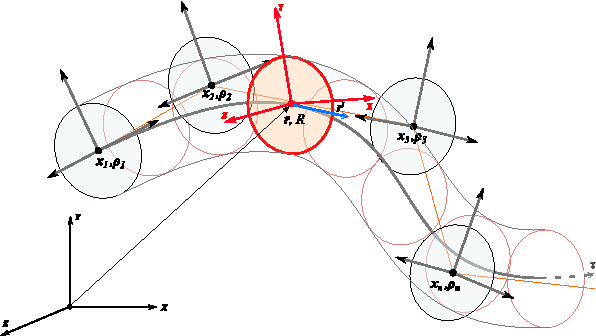
\includegraphics[width=0.75\textwidth]{beam_cosserat.pdf}
\caption{Spline discretization of the beam with independent position and rotation fields.}
\label{figdiscretize}
\end{figure}


The beam is approximated with IGA. 
To this end we assume that the beam is represented as a B-spline whose control points are nodes, each i-th node being a coordinate system $\{\avect{x}_i, \amatr{R}_i\}$ with position $\avect{x}_i \in \mathbb{R}^3$ and rotation $\amatr{R}_i \in \mathsf{SO}(3)$, as shown in Fig.~\ref{figdiscretize}.
For the rotation, however, we choose to parameterize rotation matrices $\amatr{R}$ using unit-length quaternions $\avect{\rho} \in \mathbb{H}_1$, so the configuration of each node is a compact set of 7 scalars: $\{\avect{x}_i, \avect{\rho}_i\}$.
We recall the basic properties of quaternions:
$\avect{\rho}=\rho_{0}+\avect{i}\rho_{1}+\avect{j}\rho_{2}+\avect{k}\rho_{3}$ with
$\avect{i}^2=\avect{j}^2=\avect{k}^2=\avect{i}\avect{j}\avect{k}=-1$, 
often written succinctly
$\avect{\rho}=[\rho_{s},\avect{\rho}_{v}]$ to facilitate the expression of quaternion multiplication:
\begin{align} 
\avect{\tau}\avect{\rho} = [ \tau_{s}\rho_{s} - \avect{\tau}_{v}\cdot\avect{\rho}_{v}, \;
\tau_{s}\avect{\rho}_{v} + \rho_{s}\avect{\tau}_{v} + \avect{\tau}_{v} \times \avect{\rho}_{v} ]
	\label{eq:quatproduct}
\end{align}

If needed, one can always convert quaternions into rotation matrices, as $\amatr{R}_i = \amatr{R}(\avect{\rho}_i)$, using the following property:
\begin{align}
\amatr{R}(\avect{\rho}) = \left[
	\begin{matrix}
	 \rho_0^2 + \rho_1^2 - \rho_2^2 - \rho_3^2  &  2(\rho_1 \rho_2 - \rho_3 q_0)   &  2(\rho_1 \rho_3 + \rho_2 \rho_0)  \cr
	 2(\rho_1 \rho_2 + \rho_3 \rho_0)  &  \rho_0^2 - \rho_1^2 + \rho_2^2 - \rho_3^2  &   2(-\rho_1 \rho_0 + \rho_2 \rho_3) \cr
   2(\rho_1 \rho_3 - \rho_2 \rho_0)  &  2(\rho_1 \rho_0 + \rho_2 \rho_3)  & \rho_0 ^2 -\rho_1^2 -\rho_2^2 + \rho_3^2   
	\end{matrix}
	\right]
	\label{eq:quatmatrix}
\end{align}
%
% and a similar procedure can be used, viceversa, to compute $\avect{\rho}_i = \avect{\rho}(\amatr{R}_i)

Finally we denote the quaternion conjugate as $\avect{\rho}^*$, 
with $\avect{\rho}^*=\rho_{0}-\avect{i}\rho_{1}-\avect{j}\rho_{2}-\avect{k}\rho_{3}$,
such that $\amatr{R}(\avect{\rho}_i^*)\amatr{R}(\avect{\rho}_j) = \amatr{R}(\avect{\rho}_i)^T\amatr{R}(\avect{\rho}_j) $.


\subsection{System state vectors}

The state of the system contains velocities and angular velocities of each frame $\{ \dot{\avect{x}}_i, \avect{\omega}_i \}$. We consider $\avect{\omega}_i$ expressed in frame-local coordinates. 

This means that the state of the system, for $n_n$ nodes, is given by the system-level configuration $\avect{q}$ and the system-state velocity $\avect{v}$ as: 
%
\begin{align}
\avect{q} &= \{ \avect{x}_1, \avect{\rho}_1, \avect{x}_2, \avect{\rho}_2, \ldots, \avect{x}_{n_n}, \avect{\rho}_{n_n} \} \\ 
\avect{v} &= \{ \dot{\avect{x}}_1, \avect{\omega}_1, \dot{\avect{x}}_2, \avect{\omega}_2, \ldots, \dot{\avect{x}}_{n_n}, \avect{\omega}_{n_n} \}
\end{align}
%

In both statics and dynamics analysis it happens that one has to update by updating the $\avect{q}$ configuration by applying some computed increment. For instance, in a linear static problem one has $\amatr{K} \delta\avect{q}=\avect{b}$ and $\avect{q}_{new} = \avect{q} + \delta\avect{q}$. Also numerical methods for DAEs and ODEs in dynamics proceed by performing updates on the configurations at each time step. The problem is that, within our state $\avect{q}$, positions can be updated with straight sums as 
$\avect{x}_{i,new} = \avect{x}_i + \delta\avect{x}_i$, but quaternions cannot be updated as easily. In fact doing a straight sum with a $\delta\avect{\rho}_{i} \in \mathbb{H}_1$ as in $\avect{\rho}_{i,new} = \avect{\rho}_{i} + \delta\avect{\rho}_{i}$ could invalidate the unit-length of $\avect{\rho}_{i,new}$. A more rigorous solution is to do incremental updates of quaternions using the exponential map. This requires some basic concepts of Lie algebras.


Recalling concepts of differential geometry, for an element $\amatr{R}$ in Lie group $\mathsf{SO}(3)$ and an element $\delta\amatr{\Theta}$ in the corresponding Lie algebra $\mathfrak{so}(3)$, one has
%
\begin{align}
\amatr{R}      &= \mathrm{exp}(\delta\amatr{\Theta}) \label{Rexp}\\
\delta\amatr{\Theta} &= \mathrm{log}(\amatr{R}) \label{Rlog}
\end{align}
%
One can extract the three dimensional rotation pseudovector $\delta\avect{\theta}$ from $\delta\amatr{\Theta}$ via $\delta\avect{\theta} = \text{axis}(\delta\amatr{\Theta})$, recalling that $\delta\amatr{\Theta} =  \mathrm{skew}(\delta\avect{\theta}) = \delta\tilde{\avect{\theta}}$. 
For our purposes, $\delta\avect{\theta}$ can be considered a (not necessarily infinitesimal) incremental rotation; for example in a time stepper it could be $\delta\avect{\theta} =  \avect{\omega} dt$.

For sake of compactness and performance, we avoid updating $\amatr{R}$ and we rather exploit the fact that $\mathbb{H}_1$ is a double cover of $\mathsf{SO}(3)$. Just like in \eqref{Rexp} and \eqref{Rlog}, an exponential map links $\mathbb{H}_1$, (unit  quaternions), and its Lie algebra $\mathsf{Im}(\mathbb{H})$ of \emph{pure quaternions} $\delta\avect{\rho} = [0,\delta\avect{\theta}]$:
%
\begin{align}
\avect{\rho}      &= \mathrm{exp}(\delta\avect{\rho}) \label{eq:rexp}\\
\delta\avect{\rho} &= \mathrm{log}(\avect{\rho})   \label{eq:rlog}
\end{align}
%
We can define two operators to convert pure quaternions from and to rotation pseudovectors: 
$\delta\avect{\theta}= \text{imag}([0,\delta\avect{\theta}])$,
and
$[0,\delta\avect{\theta}]= \text{pure}(\delta\avect{\theta})$.
The exponential map \eqref{eq:rexp} can be explicitly computed from $\delta\avect{\theta}$ as $\avect{\rho} = \exp (\text{pure}(\delta\avect{\theta}))$ using the following closed-form expression:
%
\begin{align}
\avect{\rho} =
\exp ([0, \delta\avect{\theta}]) = 
\left\{ 
\cos\left(\frac{||\delta\avect{\theta}||}{2}\right), 
\frac{\delta\avect{\theta} }{ ||\delta\avect{\theta}|| } \sin\left( \frac{||\delta\avect{\theta}||}{2}\right) 
\right\} \label{eq:qexponential}
\end{align}

This said, in our code we can work with increments in the following form:
%
\begin{align}
\delta\avect{q} &= \{ \delta\avect{x}_1, \delta\avect{\theta}_1, \delta\avect{x}_2, \delta\avect{\theta}_2, \ldots, \delta\avect{x}_{n_n}, \delta\avect{\theta}_{n_n} \} 
\end{align}
%
and, where one has to perform the incremental update to find $\avect{q}_{new}$, the rotational parts are incremented pre-multiplying the quaternion by an exponential map, as:
%
\begin{align}
\avect{x}_{i, new}    &= \avect{x}_i + \delta\avect{x}_i \label{eq:xinc}
\\ 
\avect{\rho}_{i, new} &= \avect{\rho}^{\delta}_{i} \avect{\rho}_{i}
\label{eq:rinc}
\end{align}
%
where one computes 
$\avect{\rho}^{\delta}_{i} = \exp ([0, \delta\avect{\theta}_{i}]) $ using \eqref{eq:qexponential}, then computes the product $\avect{\rho}^{\delta}_{i} \avect{\rho}_{i}$ using \eqref{eq:quatproduct}.
More succinctly, the incremental update is a map
$\avect{q}_{new}=\Lambda(\avect{q},\delta\avect{q})$.


In the following, for expressing formulas in a easier way, we group all the translational degrees of freedom and all the rotational degrees of freedom in two separate vectors $\avect{q}_x$ and $\avect{q}_{\rho}$, and we do the same for the increments 
$\delta\avect{q}_x$ and $\delta\avect{q}_{\rho}$:
%
\begin{align}
\avect{q}_x &= \{ \delta\avect{x}_1, \delta\avect{x}_2, \ldots, \delta\avect{x}_{n_n} \} \\
\avect{q}_{\rho} &= \{ \avect{\rho}_1, \avect{\rho}_2, \ldots, \avect{\rho}_{n_n} \} \\
\delta\avect{q}_x &= \{ \delta\avect{x}_1, \delta\avect{x}_2, \ldots, \delta\avect{x}_{n_n} \} \\
\delta\avect{q}_{\rho} &= \{ \delta\avect{\theta}_1, \delta\avect{\theta}_2, \ldots, \delta\avect{\theta}_{n_n} \}
\end{align}

\subsection{Interpolation}

In IGA, the role of FEA shape functions is done by Basis Functions of the spline.
For a given knot abscissa $\tau$ along the spline, one can compute interpolated position and gradient using Basis Functions $N_i(\tau)$ and their derivatives $\mathring{N}_i(\tau) = \frac{dN_i(\tau)}{d\tau}$, that is:
%
\begin{align}
\avect{r}(\tau)  &= \sum_i N_i(\tau) \avect{x}_i  \\
\avect{r}'(\tau) &= \frac{d\avect{r}(\tau)}{d\tau} J^{-1}_{s\tau}    \\
                 &= \sum_i \mathring{N}_i(\tau) \avect{x}_i  J^{-1}_{s\tau} 
\end{align}

Once this is computed, $\underline{\avect{\epsilon}}(\tau)$ can be computed with \eqref{eq:epsilon}.

Similarly, one would be tempted to interpolate the rotation at a given abscissa $\tau$ using a similar method, however applying directly $\avect{\rho}(\tau)  = \sum_i N_i(\tau) \avect{\rho}_i$ is not possible because the linear sum of unit quaternions does not represent, in general, a rotation. In fact, the spline interpolation of quaternions is still a debated problem and exact solutions presented in literature, such as \cite{kim1995general,kim1995c}, often lead to complex formulas that add complication and computational overhead. As a simplification we introduce an auxiliary co-rotated system $\underline{\avect{\rho}}$, for instance an average of rotations of the closest nodes, and we interpolate rotations by doing a weighted sum of rotation pseudovectors %$\text{imag}(\log(\underline{\avect{\rho}}^* \avect{\rho}_i))$, 
later recast as a quaternion using the exponential map:
%
\begin{align}
\avect{\rho}(\tau)  &= \underline{\avect{\rho}} \exp \left( \text{pure} \sum_i N_i(\tau) \text{imag}(\log( \underline{\avect{\rho}}^* \avect{\rho}_i)) \right) 
\end{align}
%
Then, the $\amatr{R}$ matrix can be computed as $\amatr{R}(\avect{\rho})$.
%
Also, the curvature $\avect{\kappa}$ is computed as:
%
\begin{align}
%\avect{\kappa}(\tau)  &=  \amatr{R}^T \sum_i J^{-1}_{s\tau} \mathring{N}_i(\tau) \text{imag}(\log(\avect{\rho}_i))  
\avect{\kappa}(\tau)  &=   \sum_i J^{-1}_{s\tau} \mathring{N}_i(\tau) \text{imag}( \log(\avect{\rho}(\tau)^* \avect{\rho}_i))
\end{align}

These allow the computation of local stresses $\avect{m}(\tau)$ and $\avect{n}(\tau)$ according to \eqref{eq:mnconstitutive}.
If a constitutive material includes damping effects, one can compute also
$\dot{\avect{\epsilon}}(\tau)= \amatr{R}^T \sum_i \mathring{N}_i(\tau) \dot{\avect{x}}_i  J^{-1}_{s\tau}$
and 
$\dot{\avect{\kappa}}(\tau) = \amatr{R}^{T} \sum_i \mathring{N}_i(\tau) \amatr{R}_i \avect{\omega}_i  J^{-1}_{s\tau}$ to be used in \eqref{eq:mnconstitutivewdamping}.


\subsection{Gauss quadrature}

As in most FEA frameworks, also in IGA the backbone of the process is the computation of three main ingredients: the vector of internal forces $\avect{f}_{int}$, the tangent stiffness matrix $\amatr{K_t}$, and the mass matrix $\amatr{M}$. Once these are computed, one can solve, for instance, linear elastic problems as $\amatr{K_t}\delta\avect{q}=\avect{f}_{ext}$, non linear elastic problems that iterate on $\amatr{K_t}\delta\avect{q}=\avect{f}_{ext}+\avect{f}_{int}$ up to convergence, explicit dynamic integration as in $\amatr{M}\ddot{\avect{q}}=\avect{f}_{ext}+\avect{f}_{int}$ and so on. 
Therefore, in the following, we present the procedure for computing these terms, starting from the most relevant part, that is the vector of internal forces $\avect{f}_{int}$.

Here we focus on computing $\avect{f}_{int}$ via typical Gauss integration. We remark that an appropriate choice of integration points must be used in order to avoid shear locking phenomena, to this end we used selective reduced integration requiring fewer quadrature points than standard integration techniques. Efficient choice of Gauss points is discussed by various authors, for instance~\cite{Hughes2010301,Hillman2015521,Adam2015732}. In fact, a more recent and efficient approach to IGA consists in using collocation instead of Gauss integration~\cite{Auricchio2013IGA,Marino2017546,weeger2018frictional}.
%We interface this Cosserat rod implementation with our C++ to leverage its contact simulation capabilities. However, it does not offer support for collocation methods.

Also, we use the same idea of FEA of computing internal forces and matrices on a per-element basis, where later all element terms will be assembled/overlapped in global system-level matrices and vectors. In this sense, in our embodiment the j-th element is the j-th span of the B-spline, so for each element we compute 
$\avect{f}_{int,j}$, and later all those per-element internal forces are assembled in a single vector
\footnote{Differently from FEA, in IGA one could compute the system-level vector without passing through intermediate per-element vectors, but here for clarity we develop our formulation on a per-element basis}.

%The potential energy of the j-th span from $s=a$ to $s=b$ is:
%
%\begin{align}
%\Pi = \frac{1}{2} \int_{a}^{b} \left( \avect{\epsilon} \avect{n} + \avect{\kappa}\avect{m} \right) ds
%- \Pi_{ext}
%\end{align}
%
Over the j-th span from $s=s_A$ to $s=s_B$ the weak form of the equilibrium reads:
%
\begin{align}
\delta\Pi = 
 \int_{s_A}^{s_B} \left( \delta\avect{\epsilon}_a \avect{n}_a + \delta\avect{\kappa}_a \avect{m}_a \right) ds 
-\int_{s_A}^{s_B} \left( \delta\avect{x}_a \underline{\avect{n}}_a + \delta\avect{\theta}_a\underline{\avect{m}}_a \right) ds 
\end{align}
%
Recalling \eqref{eq:epsilon}, evaluating its increment and referring it to the global coordinates:
%reissner: 12a/ 12b from 8 a/b
\begin{align}
\delta\avect{\epsilon}_a &= \delta\avect{r}'_a - \delta\avect{\theta}_a \times \avect{r}'_a  
\end{align}

So, at a point at abscissa $\tau$ along the spline, $\delta\avect{\epsilon}$ and $\delta\avect{\kappa}$ can be expressed using interpolation of the B-spline given the following terms:
%
\begin{align}
\delta\avect{r}'_a       &= \sum_i J^{-1}_{s\tau} \mathring{N}_i \delta\avect{x}_i    \\
\delta\avect{\kappa}_a   &= \sum_i J^{-1}_{s\tau} \mathring{N}_i \amatr{R}_i \delta\avect{\theta}_i \\
\delta\avect{\theta}_a   &= \sum_i      {N}_i \amatr{R}_i \delta\avect{\theta}_i
\end{align}

We rewrite the weak equilibrium introducing the vector of internal forces
%
\begin{align}
\delta\avect{q}^T_j \avect{f}_{int,j} -  \delta\avect{q}^T_j \avect{f}_{ext,j} = \avect{0} 
\end{align}

where $\avect{f}_{int,j}$ and $\avect{f}_{ext,j}$ are the internal and external forces acting on the $j$-th node.

Looking at the expressions above, one can write the expression of the contribution from the $i$-th control node to $\avect{f}_{int,j}$ as an integral in $s$ arc-length coordinate:
%
\begin{align}
\avect{f}_{int,j,i} = \int_{s_A}^{s_B} 
 \left[  
	\begin{array}{cc}
	 J^{-1}_{s\tau} \mathring{N}_i  \amatr{I}  &  N_i \amatr{R}_i \tilde{\avect{r}}'\\
	 0                           & J^{-1}_{s\tau} \mathring{N}_i \amatr{R}_i 
	\end{array}
	\right]^T
	\left[  
	\begin{array}{c}
	 \avect{n}_a  \\
	 \avect{m}_a  
	\end{array}
	\right]
	ds
\end{align}

The integral is computed with a sum over $n_{gp}$ Gauss points, so we introduce Gauss point weights $w_k$, jacobians $J_{\tau\zeta} = \frac{d\tau}{d\zeta}$ where $\zeta \in [-1,+1]$ is the coordinate used for Gauss quadrature. Because of change of coordinates, we also have to multiply the integrand by $J_{s\tau}$, so some jacobians will simplify as $J^{-1}_{s\tau} J_{s\tau}=1$. 
Finally one has:
%
\begin{align}
\avect{f}_{int,j,i} = \sum_k^{n_{gp}} 
 w_k J_{\tau\zeta}
 \left[  
	\begin{array}{cc}
	 \mathring{N}_i \amatr{I}   & J_{s\tau} N_i \amatr{R}_i \tilde{\avect{r}}'\\
	 0                     & \mathring{N}_i \amatr{R}_i 
	\end{array}
	\right]^T
	\left[  
	\begin{array}{c}
	 \avect{n}_a  \\
	 \avect{m}_a  
	\end{array}
	\right]
	\label{fint}
\end{align}

Here all the terms of the integrand (namely, $N_i$, $\mathring{N}_i$, $J_{s\tau}$, $\tilde{\avect{r}}'$, $\avect{n}_a$ and $\avect{m}_a$) must be computed for the k-th knot abscissa $\tau_k =  \left(\frac{s_B-s_A}{2} \zeta_k + \frac{s_B+s_A}{2}\right)$ where $\zeta_k$ is one of the $n_{gp}$ tabulated abscissas for Gauss integration, i.e. coupled to the corresponding weight $w_k$. By the way one can see that $J_{\tau\zeta} = \frac{s_B-s_A}{2}$.

We remark that control points will affect neighbouring spans (elements) hence  terms $\avect{f}_{int,j,i}$ from different spans will overlap and must be summed to obtain $\avect{f}_{int,j}$.

The number of nodes influencing a single span increases with the spline order. IGA spline Basis Functions can be considered like shape functions affecting more knot spans, combining each other in the shared segments of support. For this reason an higher spline order leads to more overlapped Basis Functions, while increasing the element order in FE analysis adds nodes within the element but internal nodes do not affect adjacent elements. This leads to a band-diagonal stiffness matrix whose band width increases with the spline order, as opposed to traditional FE elements characterized by a block-diagonal stiffness matrix whose blocks overlap only at the boundary nodes.

\section{Stiffness, mass and damping matrices}

For the time integration of the equations of motion, the mass matrix is needed. If implicit integration schemes are used, also the tangent stiffness and damping matrices are required.

In our implementation we use a lumped mass matrix where each $i$-th IGA control point has an atomic mass $m_i$ and a tensor of inertia $I_i \in \mathbb{R}^{3\times3}$. This has a computational advantage with respect to the explicit quadrature of the beam shape, because the tensor of inertia $I_i=\text{diag}(I_{xx_i},I_{yy_i},I_{zz_i})$ is diagonal and constant as a consequence of the fact that we assumed angular velocities $\avect{\omega}_i$ to be expressed in the local coordinate system. Values of $m_i, I_{xx_i}, I_{yy_i}, I_{zz_i}$ can be computed from the geometry of the section and from the density of the material.

The tangent stiffness matrix and the damping matrix are computed by numerical differentiation of $\avect{f}_{int}$.
%
\begin{align}
\amatr{K_t} 
= -\nabla_{\avect{q}} \avect{f}_{int} 
= - \left[  \frac{\partial\avect{f}_{int}}{\partial\avect{q}} \right], 
\quad
\amatr{R_t} 
= -\nabla_{\avect{v}} \avect{f}_{int} 
= - \left[  \frac{\partial\avect{f}_{int}}{\partial\avect{v}} \right]
	\label{KRmatr}
\end{align}

Since the procedure for computing \eqref{fint} is quite simple, the computational overhead is not excessive with respect to an analytic evaluation of the matrix, yet it has the useful property of being of general validity even when using black-box nonlinear constitutive laws for materials. For a practical implementation, for the sake of high performance, one should exploit the sparsity pattern of $\amatr{K_t}$. In detail, the numerical differentiation operates on a per-span basis, to obtain per-span stiffness matrices $\amatr{K_t}_{j}$ that are summed afterward to obtain the large and sparse $\amatr{K_t}$ system-level matrix.


\section{Contacts}

\begin{figure}[ht]
\centering
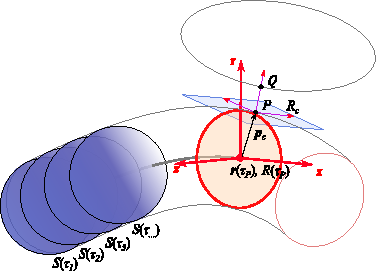
\includegraphics[width=0.55\textwidth]{beam_cosserat_collision.pdf}
\caption{Sampling the beam with contact shapes (proxies) for fast collision detection.}
\label{figcontact}
\end{figure}

We developed a framework for simulating contacts between moving parts, either beams and other objects (rigid bodies, other finite elements, etc.). 

When targeting complex scenarios with thousands of elements, we experienced that an efficient approach is to sample the rod with simple collision geometries that can be easily handled by fast collision algorithms. For example a rod with a circular section can be approximated with invisible collision spheres $S_i$, evenly spaced along the beam centerline, at given parametric abscissas $\tau_i$, as shown in Fig.~\ref{figcontact}. Those proxies are passed to the collision engine that computes candidate collision points at each time step: to this end we use a Sweep-And-Prune (SAP) broad-phase optimization that allows a near linear-time complexity even in case of many shapes, and a Gilbert-Johnson-Keerthi~(GJK) algorithm for the narrow-phase. 

The narrow-phase returns a variable number of candidate contact pairs, each represented by two points $\avect{P}$ and $\avect{Q}$ belonging to two colliding shapes, and a coordinate system $\amatr{R_c}$ whose $x$ axis represent the contact normal. We assume that the contact distance $\Phi=|\avect{P}-\avect{Q}|$ is differentiable. The distance vector, in the contact coordinates, is $\avect{D}=\amatr{R_c}^T(\avect{P}-\avect{Q})$.

In order to write the equation of motion in the following section, we need to express the relative speed of the two points, $\avect{u}=\amatr{R_c}^T(\dot{\avect{P}}-\dot{\avect{Q}})$ as a function of generalized coordinates $\avect{v}$.

Assuming point $\avect{P}$ belongs to a beam, we can recover $\tau_P$, the abscissa at which the colliding shape was sampled.
This allows the immediate 
\footnote{An optional refinement can happen at this point: since the collision shape -a sphere, a capsule...- was only an approximation of the smoothly bent surface of the beam, one can iteratively correct the (discrete-sampled) contact abscissa in order to satisfy $\avect{P}(\tau_P)=\avect{r}(\tau_B)+\amatr{R}(\tau_P)\avect{p}_{c}$ until the position of the contact point in the beam section frame, $\avect{p}_{c}$, has perfectly zero off-section value: $p_{c,x}=0$}
computation of $\amatr{R}(\tau_P)$, the rotation of the section at the contact, and $\avect{p}_{c}$, the position of the contact point in the section coordinate system, as in $\avect{P}(\tau_P)=\avect{r}(\tau_P)+\amatr{R}(\tau_P)\avect{p}_{c}$.

Taking the time derivative, simplifying for $\dot{\avect{p}}_c=0$ and recalling the spline Basis Functions:
%
\begin{subequations}
\begin{align}
\dot{\avect{P}}(\tau_P) &=
 \dot{\avect{r}}(\tau_B) +
 \dot{\amatr{R}}(\tau_P) \avect{p}_c +
 \amatr{R}(\tau_P) \dot{\avect{p}}_c \\
 &=\sum_i{N_i(\tau_P)\dot{\avect{x}}_i } +
  \amatr{R}(\tau_P) \tilde{\avect{\omega}}(\tau_P) \avect{p}_{c} + 0 \\
 &=\sum_i{N_i(\tau_P)\dot{\avect{x}}_i } 
  -\amatr{R}(\tau_P) \tilde{\avect{p}}_{c} \avect{\omega}(\tau_P) \\
 &=\sum_i{N_i(\tau_P)\dot{\avect{x}}_i } -
  \sum_i{N_i(\tau_P)\amatr{R}(\tau_P) \tilde{\avect{p}_{c}} \avect{\omega}_{i}} \label{eq:jaco}
\end{align}
\end{subequations}


At this point it is possible to write the contact speed of the $k$-th contact using generalized coordinates, 
$\avect{u}_k=\nabla_{\avect{v}}^T\amatr{D}_k \avect{v}$,
where the jacobian $\nabla_{\avect{v}}^T  \amatr{D}_k \in \mathbb{R}^{3 \times n_v}$ has a sparse structure with two blocks:
\begin{equation}
\nabla_{\avect{v}}^T\amatr{D_k} =
\left[\dots, \nabla_{\avect{v}}^T\amatr{D_k}_P, \dots, \nabla_{\avect{v}}^T\amatr{D_k}_Q, \dots \right].
\end{equation}
In detail, from \eqref{eq:jaco} one has
%
\begin{multline}
\nabla_{\avect{v}}^T\amatr{D_k}_P = 
 \Big[ 
  N_1(\tau_P) \amatr{R_c}^T,
  -N_1(\tau_P) \amatr{R_c}^T \amatr{R}(\tau_P) \amatr{\tilde{p_{c}}}, \\
  N_2(\tau_P) \amatr{R_c}^T, 
  -N_2(\tau_P) \amatr{R_c}^T \amatr{R}(\tau_P) \amatr{\tilde{p_{c}}}, \\
  \dots,
  N_n(\tau_P) \amatr{R_c}^T,
  -N_n(\tau_P) \amatr{R_c}^T \amatr{R}(\tau_P) \amatr{\tilde{p_{c}}}
 \Big]
 \label{eq:jacodetail}
\end{multline}
%
whereas an equivalent expression holds for $\nabla_{\avect{v}}^T\amatr{D_k}_Q$ if also $\avect{Q}$ belongs to a beam 
\footnote{For instance, if $\avect{Q}$ belongs to a rigid body, the corresponding jacobian block has a simpler expression: 
$\nabla_{\avect{v}}^T\amatr{D_k}_Q=
\left[ 
-\amatr{R_c}^T,  \amatr{R_c}^T \amatr{R_b} \amatr{\tilde{q_{c}}}
\right]$ where $\amatr{R_b}$ is the rotation of the body and $\avect{q}_{c}$ is the position of $\avect{Q}$ in body local coordinates.}.

As a special case, very thin beams have $||\avect{p_{c}}||\approx 0$ hence $-N_n(\tau_P) \amatr{R_c}^T \amatr{R}(\tau_P) \amatr{\tilde{p_{c}}}$ terms could be removed from the jacobian in sake of performance. 

Finally, it is possible to group all $n_c$ contact jacobians in a system-level sparse matrix $\nabla_\avect{v}^T \avect{D} \in \mathbb{R}^{3n_c \times n_v}$.


\section{Time stepping and implementation}

In the most general setting, we assume that the system is made by a several IGA beams, as well as other finite elements and rigid bodies, and we assume that all their states are grouped in the system-level vectors  $\avect{q}$ and $\avect{v}$. Also, we assume that the configuration is subject to holonomic-rheonomic constraint equations $\avect{C}(\avect{q},t) = \avect{0}$. Differentiation of constraints leads to 
$\frac{\partial \avect{C}}{\partial \avect{q}} \frac{\partial \avect{q}}{\partial t} + \frac{\partial \avect{C}}{\partial t} = \avect{0}$, 
that is 
$\nabla_\avect{v}^T \avect{C} \avect{v} + \avect{C}_t = \avect{0}$
where
$\nabla_\avect{v}^T \avect{C} = \frac{\partial \avect{C}}{\partial \avect{q}} \Gamma(\avect{q})$ is the constraint jacobian, $\Gamma(\avect{q})$ is a linear operator for 
$\dot{\avect{q}} = \Gamma(\avect{q}) \avect{v}$, 
and $\avect{C}_t$ is a null term in case of scleronomic constraints, but can appear in case of time-dependant constraints (motors, imposed trajectories, etc.).

We perform time integration either with implicit integrators \footnote{HHT \cite{JayNegrut2007} or Newmark \cite{negrutGavrea2005} in our implementation, here not described for compactness.} for smooth Differential-Algebraic-Equations (DAE), or with a custom time stepper for non-smooth DVI.
The latter allows also an efficient treatment of contacts. In fact, if one wants to simulate contacts in the framework of conventional smooth dynamics, in most cases contact constraints would be dealt with regularization, i.e. penalty functions that would require very short time steps. On the other hand, the DVI approach embeds the set-valued non-smooth nature of contact forces directly in the formulation~\cite{negrut2018posing}.
At $l$-th time step we solve:
\begin{align}
    \begin{bmatrix}
    \amatr{H} & \nabla_\avect{v}  \avect{C} & \nabla_\avect{v} \avect{D}\\
    \nabla_\avect{v}^T \avect{C} & 0 & 0 \\
    \nabla_\avect{v}^T \avect{D} & 0 & 0 
    \end{bmatrix}
    \begin{pmatrix}
    \avect{v}^{(l+1)} \\
    \avect{\lambda}_C \\
    \avect{\lambda}_D \\
    \end{pmatrix}
    -
    \begin{pmatrix}
    \amatr{H}   \avect{v}^{(l)} + h(\avect{f}_{int}+\avect{f}_{est})\\
    -\frac{1}{h}\avect{C}(\avect{q},t) - \avect{C}_t\\
    -\frac{1}{h}\avect{\Phi}(\avect{q})
    \end{pmatrix}
    = 
    \begin{pmatrix}
    \avect{0}\\
    \avect{0}\\
    \avect{y}
    \end{pmatrix} \label{eq:dvi}
    \\
    \avect{y} \in \Upsilon^* \bot \avect{\lambda}_D \in \Upsilon  \label{eq:complementarity} 
    \\
    \avect{q}^{(l+1)}=\Lambda(\avect{q}^{(l)},h\avect{v}^{(l+1)}) \label{eq:increment}
\end{align}
%
where $\amatr{H}=\amatr{M}+h^2\amatr{K}_t+h\amatr{R}_t$ is a sparse matrix, $h$ is the time step, contact jacobians are computed as in \eqref{eq:jacodetail}, $\Upsilon = \oplus_i \Upsilon_i$ is the Cartesian product of all Coulomb friction cones generated by contacts, and 
$\Upsilon^* = 
\left \{\avect{\lambda}_D \in \Upsilon^*: \langle  \avect{\lambda}_D, \avect{z} \rangle \geq 0 \quad \forall \avect{z}\in \Upsilon  \right \}
= \oplus_i \Upsilon_i^*$ 
is its dual. Finally, \eqref{eq:increment} is updated with exponential maps as in \eqref{eq:xinc}-\eqref{eq:rinc}.

In absence of contacts, it can be demonstrated that the algorithm \eqref{eq:dvi}-\eqref{eq:increment} simplifies to a backward Euler linearly implicit integrator, of whom it inherits the same properties of first order accuracy in time and L-stability. If higher order accuracy or less numerical damping is needed, recent research demonstrated the possibility of second-order DVI time steppers at the cost of additional complexity in the implementation \cite{bruls2018constraints}.

The problem \eqref{eq:dvi}-\eqref{eq:complementarity} is a Second-Order Cone Complementarity Problem (SO-CCP) with unknowns $\avect{v}^{(l+1)}$, the speed at the end of time step, and $\avect{\lambda}$, the reaction impulses in contacts or bilateral constraints. The convex cone complementarity problem is also a special case of a Variational Inequality (VI), hence the DVI acronym~\cite{StPa08}.

The complementarity constraint \eqref{eq:complementarity} introduces a major numerical difficulty, however the monolithic SO-CCP \eqref{eq:dvi}-\eqref{eq:complementarity} can be solved efficiently using the primal-dual interior point method that we presented in~\cite{MANGONI2018351} and that we implemented in C++.

Although the DVI integrator \eqref{eq:dvi}-\eqref{eq:increment} is stable also when using large time steps, we remark that there are scenarios where the time step must be extremely short anyway, for example because one wants to simulate collisions between very thin beams, a case that requires small steps in order to avoid tunneling and aliasing effects in the computation of contact points; in such cases, the advantage of using the DVI is less evident. 

Comparing this non-smooth DVI integrator to conventional smooth explicit integrators, one can see that DVI requires more computational effort per each time step, because of the SO-CCP overhead. On the other hand, explicit integrators require a much larger number of time steps to achieve stability, depending on how stiff is the contact formulation. 

Comparing the DVI integrator to conventional smooth implicit integrators embedded with penalty formulations leads to similar conclusions: the SO-CCP solver overhead is still higher than the few linear system solves required in the Newton iterations of implicit steppers, but on the other side the total number of time steps can be smaller. Implicit solvers, in fact, could use large time steps as the DVI, but the highly non-linear nature of the contact forces often impair their performance to the point that they need short time steps anyway. 

In general, since the SO-CCP solution dominates the overall computational effort per each time step of the DVI, the efficiency of the DVI method respect to smooth integrators depends mostly on how optimized is the SO-CCP solver. 
In order to maximize the computational performance, the inner loop of our interior-point method leverages the MKL parallel direct solver from Intel. As an alternative, we tested also CVXOPT, a Python library for large-scale cone programming, again based on an interior-point method~\cite{andersen2011interior}. 

%In conclusion the total CPU time used to compute a simulation with DVI, hence its overall efficiency, is less -or more- than one used by smooth integrators depending on the following factors that change from case to case: how stiff is the contact penalty (steel-like structures are more likely to be efficiently solved by DVI, rather than soft structures), how fast the SO-CCP solver can compute the solution (objects with odd mass scaling, for instance, are known to require longer CPU times in our SO-CCP solver, and some implementations of SO-CCP solvers converge much faster than others), presence of collisions between very thin objects.



\section{Numerical tests}

% REMOVED SUBSECTION ON LINEAR STATICS (CANTILEVER
% BENCHMARK WITH TABLES) AS IT SEEMS TO MUCH. 
% REMOVE COMMENT IN FRONT OF \input{...} 
% TO ENABLE AGAIN, IF NEEDED. ALESSANDRO.
%
% \input{"chapter_cantilever.tex"}

\subsection{The ring bending test}

This is a classical benchmark where a cantilever beam is subject to a concentrated torque $T$ acting on the tip to obtain a ring bending deformation. Since the length of the neutral axis is constant under pure bending, the initial beam length \emph{L} must be equal to the final circumference, hence the curvature radius must be $\rho = \frac{L}{2\pi}$.
For a linear elastic rod it holds
$\rho = \frac{E I}{T}$, so the torque required to obtain a perfect circle must be 
%
\begin{equation}
T = \frac{2\pi EI}{L} \nonumber
\end{equation}

Because of the large deformations, we performed a non-linear static analysis where the torque value has been increased gradually to avoid divergence. Our simulations converge consistently with the analytical solution, as shown in Fig.~\ref{figringbending}.

\begin{figure}[ht]
\centering
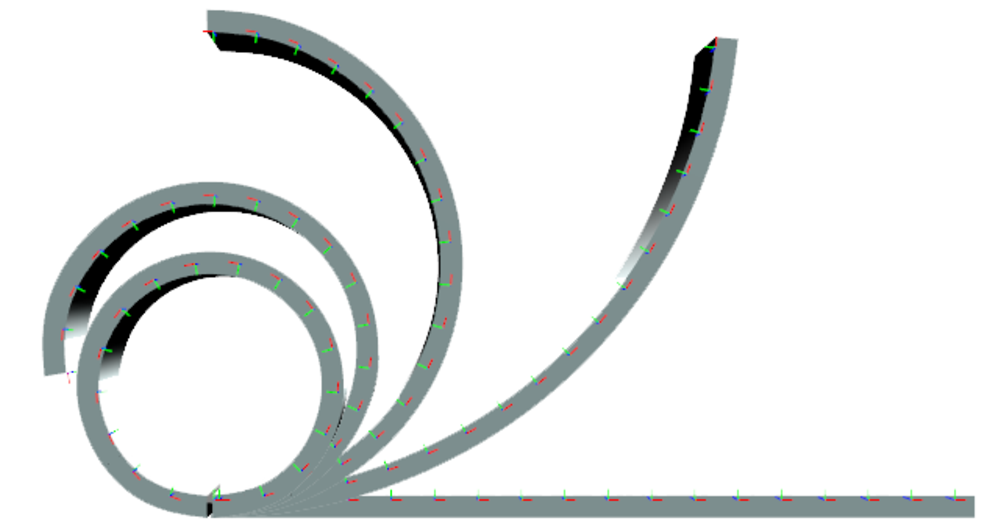
\includegraphics[width=0.65\textwidth]{benchmark_RingBending/bending_progression.pdf}
\caption{Progression of ring bending}
\label{figringbending}
\end{figure}


\subsection{Princeton beam experiment}

A thin beam, depicted in Fig.~\ref{figB1setup}, is subject to large deformations and large rotations because of a tip load at $E$, for different angles $\theta$. A non-linear analysis shows that, for large displacements, a strong twisting action couples to the bending action, hence obtaining out-of-plane displacements even if the load is vertical.

Three loading conditions are tested: $P_1 = 4.448$N, $P_2 = 8.896$N,
and $P_3 = 13.345$N, for $\theta$ ranging in the $[0^\circ,90^\circ]$ interval.
The beam has length $L = 0.508$m, section height $H = 12.77$mm, section thickness $T = 3.2024$mm, Young modulus $E = 71.7$GPa, $\nu = 0.31$, $G = E \frac{(1 + \nu)}{2} = 27.37$GPa. 

Because of the geometric nonlinearities, the solver must perform Newton-Raphson steps
before obtaining a zero residual in the equations of static equilibrium.
% For very large nonlinearities, a continuation strategy might help the convergence of the Newton-Raphson solver.

Results in Figs.~\ref{figB1r1}, \ref{figB1u2} and \ref{figB1u3} show a good agreement
between the present IGA formulation and reference data~\cite{BAUCHAU-2014-IMSD}. In detail, there is a good agreement with other geometrically-exact beam formulations (non IGA-based) discussed in~\cite{BAUCHAU-DYMORE} for Dymore and in~\cite{FV-AIAA} for MBDyn, 
as well as an agreement with the experimental results
in~\cite{DOWELL-1975-PRINCETON-1194,DOWELL-1975-PRINCETON-1257}, obtained with a beam made with 7075 aluminium alloy.

\begin{figure}[ht]
 \begin{minipage}[b]{0.48\linewidth}
    \centering
    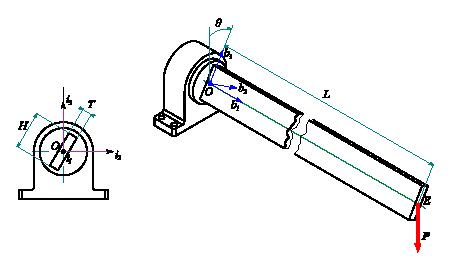
\includegraphics[width=0.99\textwidth]{benchmark_princeton/setup_princeton.eps}
    \caption{Setup of the benchmark for the Princeton beam experiment.}
    \label{figB1setup}
 \end{minipage}
 \hspace{0.4cm}
 \begin{minipage}[b]{0.48\linewidth}
    \centering
    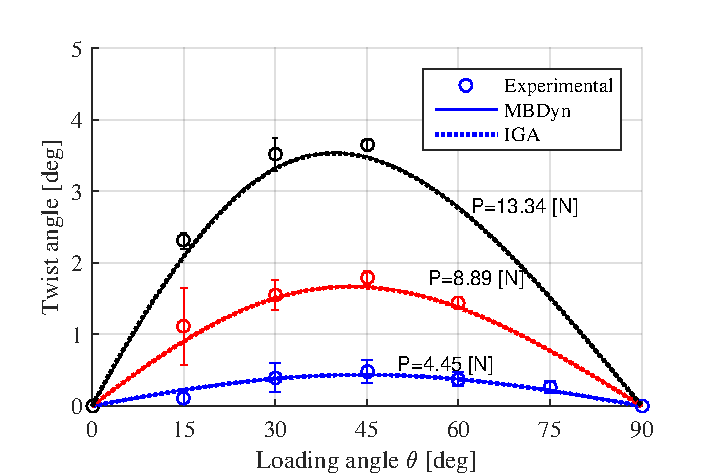
\includegraphics[width=0.99\textwidth]{benchmark_princeton/benchmark_princeton_r1.pdf}
    \caption{Twist rotation of the beam for the Princeton experiment.}
    \label{figB1r1}
 \end{minipage}
\end{figure}

\begin{figure}[ht]
 \begin{minipage}[b]{0.48\linewidth}
    \centering
    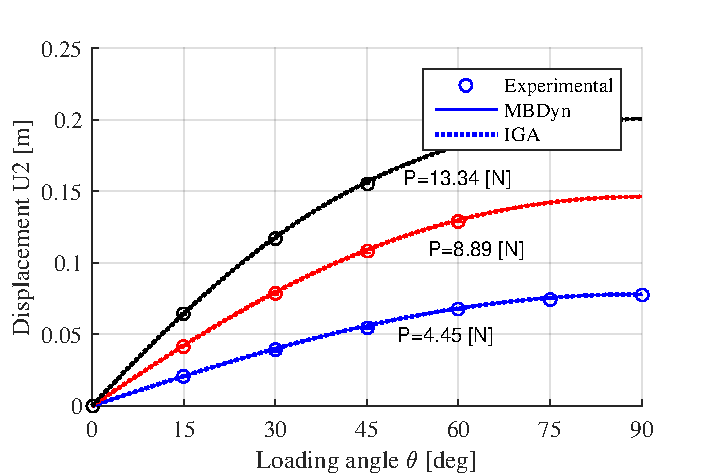
\includegraphics[width=0.99\textwidth]{benchmark_princeton/benchmark_princeton_u2.pdf}
    \caption{Flapwise displacement at the beam tip versus loading angle for three loading conditions.}
    \label{figB1u2}
 \end{minipage}
 \hspace{0.4cm}
 \begin{minipage}[b]{0.48\linewidth}
    \centering
    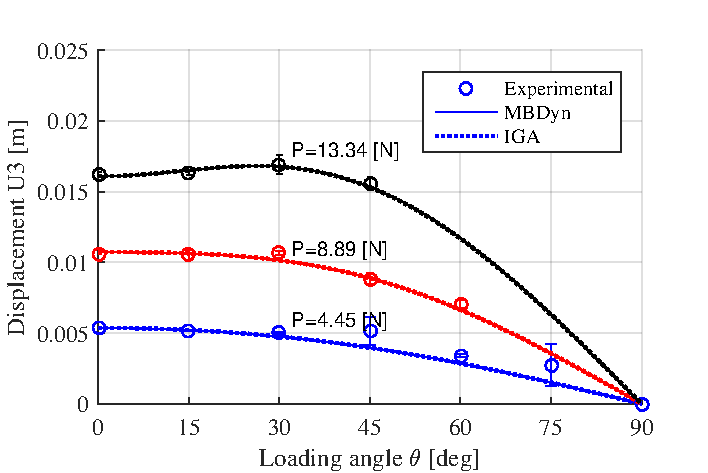
\includegraphics[width=0.99\textwidth]{benchmark_princeton/benchmark_princeton_u3.pdf}
    \caption{Chordwise displacement at the beam tip versus loading angle for three loading conditions.}
    \label{figB1u3}
 \end{minipage}
\end{figure}



% REMOVED SUBSECTION ON MODDAL ANALYSIS
% IT SEEMS TO MUCH. REMOVE COMMENT IN FRONT
% OF \input{...} TO ENABLE IF NEEDED. 
%\input{"chapter_modal.tex"}

\subsection{Jeffcott rotor}

\begin{figure}%[ht]
 \begin{minipage}[b]{0.4\linewidth}
    \centering
    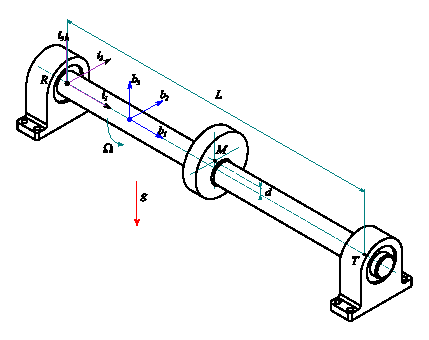
\includegraphics[width=0.99\textwidth]{benchmark_jeffcott/setup_jeffcott.eps}
    \caption{Setup of the unbalanced rotating shaft benchmark.}
    \label{figJRsetup}
 \end{minipage}
 \hspace{0.4cm}
 \begin{minipage}[b]{0.55\linewidth}
    \centering
	\psfrag{u[m]}{\tiny $\boldsymbol{u}_2$, $\boldsymbol{u}_3$ [m]}
    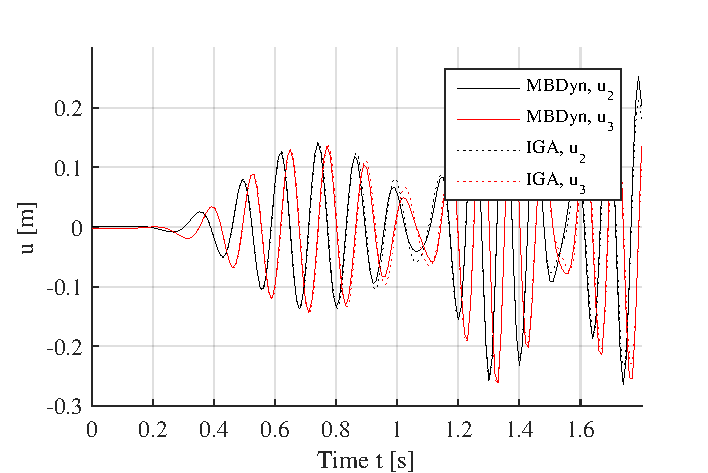
\includegraphics[width=0.99\textwidth]{benchmark_jeffcott/benchmark_jeffcott.pdf}
    \caption{Mid-point transverse displacement of unbalanced rotating shaft.}
    \label{figJRdisp}
 \end{minipage}
\end{figure}

This benchmark explores the reliability of the numerical method in the nonlinear dynamical analysis
of a flexible system rotating at finite angular velocity.
A rotating unbalanced shaft of length $L$ = \SI{6}{\meter} is integrated in time.
As shown in Fig.~\ref{figJRsetup}, a rigid disk is connected to the shaft at mid-span,
above the reference shaft axis by an offset $d$ = \SI{0.05}{\meter}.
The shaft is made of steel (density $\rho$ = 7800kg/m$^3$,
Young's modulus $E$ = \SI{210}{\giga\pascal}, Poisson's ratio $\nu$ = 0.3).
The cross section is annular ($r_i$ = \SI{0.045}{\meter}, $r_o$ = \SI{0.05}{\meter}).
The mass of the disk is $m_d$ = 70.573kg,
the radius is $r_d$ = 0.24m,
and the thickness is $t_d$ = 0.05m.
The system is subjected to gravity ($g$ = \SI{9.81}{\meter\per\square\second})
directed transversely.
The end $R$ of the shaft is connected to the ground
by a cylindrical joint (displacement along and rotation
about the shaft's axis are permitted).
The end $T$ is supported by a revolute joint;
the relative angular velocity about the shaft axis is prescribed
as a function of time, % $\omega = \Omega(t)$:
\[
\Omega(t) = \left\{
\begin{array}{lr}
	A_1 \omega (1 - \cos(\pi t / T_1))/2 & 0 \le t \le T_1
	\\
	A_1 \omega & T_1 < t \le T_2
	\\
	A_1 \omega + (A_2 - A_1) \omega (1 - \cos(\pi (t - T_2)/(T_3 - T_2)))/2 & T_2 < t \le T_3
	\\
	A_2 \omega & T_3 < t
\end{array}
\right.
\]
with
$A_1$ = 0.8,
$A_2$ = 1.2,
$T_1$ = 0.5s,
$T_2$ = 1s,
$T_3$ = 1.25s, and
$\omega$ = \SI{60}{\radian\per\second}, close to the first natural frequency of the system.
%
The shaft accelerates from zero and passes from sub-critical to super-critical regime;
when passing through the first natural bending frequency of the system,
lateral oscillations occur and significant forces take place, as predicted
by the linear theory of unbalanced rotors.

Results plotted in~Fig.\ref{figJRdisp} for the case of a 3rd order IGA with nine nodes, using a second order implicit time stepping integrator, show a good agreement with reference results obtained with MBDyn.


\subsection{Lateral buckling}

This is a benchmark that tests the beam formulation in the context of a dynamical problem of difficult integration.

In detail, a flat beam is bent in its plane of highest flexural rigidity, up to the point where lateral buckling is instantly triggered. In a quasi-static non-linear analysis,  
results are visible in Fig.~\ref{figB2static}. In the context of dynamics, when buckling occurs, the beam snaps laterally and twists, inducing highly oscillatory motions. The IGA beam discussed in this paper can capture the nonlinear nature of this phenomena.

\begin{figure}%[ht]
 \begin{minipage}[b]{0.48\linewidth}
    \centering
    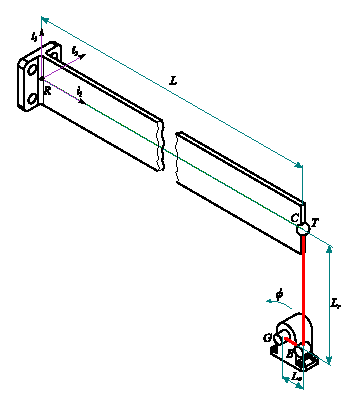
\includegraphics[width=0.70\textwidth]{benchmark_buckling/setup_buckling.eps}
    \caption{Setup of the benchmark for lateral buckling dynamics.}
    \label{figB2setup}
 \end{minipage}
 \hspace{0.4cm}
 \begin{minipage}[b]{0.48\linewidth}
    \centering
    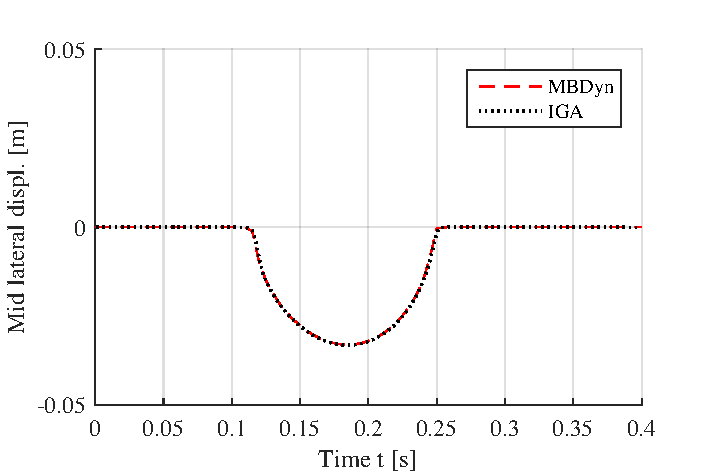
\includegraphics[width=0.99\textwidth]{benchmark_buckling/benchmark_buckling_disp_static.pdf}
    \caption{Static displacement of the beam along $i_2$, at the mid point.}
    \label{figB2static}
 \end{minipage}
\end{figure}

As depicted in Fig.~\ref{figB2setup}, a $RC$ beam with length $L=1$m and rectangular section  $H=100$mm, $B=10$mm, is clamped at the $R$ end point.
The snapping is caused by a tip load at $C$, generated by mean of a rotating crank $GB$ and a vertical rod $TB$, with a spherical joint in $C$ and a revolute joint in $B$. An initial imperfection is simulated by introducing a small offset $d=0.1$mm in the off-plane direction $i_2$ between the crank and the vertical bar. 

The crank has length $L_c=0.05$m and its circular section has diameter $D_r=24$mm, the vertical rod 
has length $L_r=0.25$m and its circular section has diameter $D_r=48$mm.
The rotation of the crank is enforced by a prescribed motion function 
$\phi_c(t)= \pi(1-\cos(\pi t/T_c) )/2$, with $T_c = 0.4$s, 
then after $t>T_c$ it holds $\phi_c(t)=\pi$.

All parts have Young modulus $E = 73$GPa and Poisson ratio $\nu = 0.3$. For the three beams, inertia values $I_{zz}$ and $I_{yy}$ and torsion constants $J$ are computed using formulas available in classical textbooks. 

\begin{figure}%[ht]
  \begin{minipage}[b]{0.48\linewidth}
    \centering
    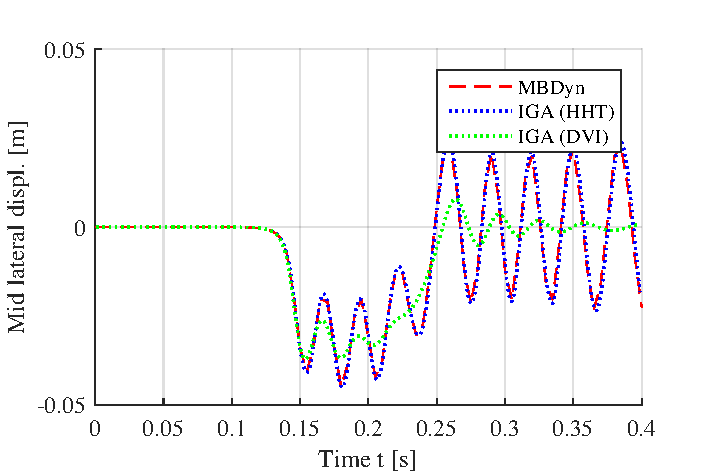
\includegraphics[width=0.99\textwidth]{benchmark_buckling/benchmark_buckling_disp.pdf}
    \caption{Displacement of the beam along $i_2$, at the mid point.}
    \label{figB2disp}
 \end{minipage}
 \hspace{0.4cm}
 \begin{minipage}[b]{0.48\linewidth}
    \centering
    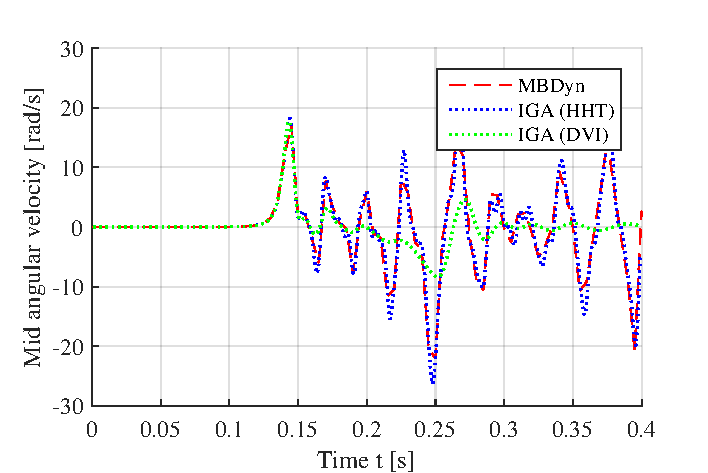
\includegraphics[width=0.99\textwidth]{benchmark_buckling/benchmark_buckling_vel.pdf}
    \caption{Angular velocity of the beam, at the mid point.}
    \label{figB2wvel}
  \end{minipage}
\end{figure}

In our tests the crank and the rod are modeled with 4 nodes each, using first order IGA beams, whereas the $RC$ beam is modeled with 12 nodes, using third order IGA beams.

We performed the dynamical analysis both with a conventional HHT time integrator and with the DVI time stepper of \eqref{eq:dvi}-\eqref{eq:complementarity}.
Comparing the results with the reference data obtained with MBDyn in Figs.~\ref{figB2disp} and \ref{figB2wvel}, a remarkable fact is that the lateral buckling is triggered exactly at the same moment for all the formulations, and the resulting oscillations have the same period. 
However, as expected, the DVI time stepper introduces some numerical damping. In fact, in scenarios that do not involve frictional contacts as in this benchmark, the conic complementarity constraint \eqref{eq:complementarity} disappears and the DVI time stepper boils down to a linearly-implicit first-order scheme, hence it shows the same damping effect of an implicit Euler method~\cite{TasoraAnitescuCMAME10}. When using the HHT second-order implicit time integrator, results are affected by numerical damping to a lower degree. The drawback of the numerical damping in the DVI method can still be accepted when its superior stability and its efficiency in contact problems are attractive, as shown in the following example.


\subsection{Contacts with rigid body}

This benchmark shows that the proposed IGA beam performs well in a dynamical simulation with complex spatial contacts, especially when using the non-smooth formulation embedded in the DVI time stepper. 
A bundle of IGA beams has been fixed between two shafts, one of which is rotating at constant speed. A fixed central rod has been added, so that it will be wrapped by the IGA beams during the simulation, see Fig.~\ref{fig:contact}.

The bundle consists in a set of eight beams, each being an IGA beam of third order with \num{57} nodes, for a total length of~\SI{0.5}{\meter}. The section is circular with a diameter of \SI{0.01}{\meter}, the Young modulus is $E=\SI{0.5}{\giga\pascal}$, the shear modulus $G=\SI{0.35}{\giga\pascal}$, the density is $\rho=\SI{1000}{\kilogram\per\cubic\meter}$. The internal cylinder diameter is~\SI{0.5}{\meter}, while the beams are distributed on a circular pattern of diameter~\SI{0.5}{\meter}. The rotation speed is~\SI{1}{\radian\per\second}.

The interior-point solver used in this simulation is request to achieve a tolerance of~\num{1d-10} over the residuals and complementarity gap.

%Additional information can be found in~Tab.\ref{tab:torque_data}.

%\begin{table}[ht]
%\centering
%    \begin{tabular}{lc}
%    \toprule
%    Parameter & Value \\
%    \midrule
%    Young Modulus & \SI{0.5}{\giga\pascal} \\
%    Shear Modulus & \SI{0.35}{\giga\pascal} \\
%    Density & \SI{1000}{\kilogram\per\cubic\meter} \\
%    \bottomrule
%    \end{tabular}
%\caption{IGA beam parameter for contact benchmark.}
%\label{tab:torque_data}
%\end{table}

\begin{figure}[ht]
    \centering
    \begin{subfigure}[b]{0.475\textwidth}
        \centering
        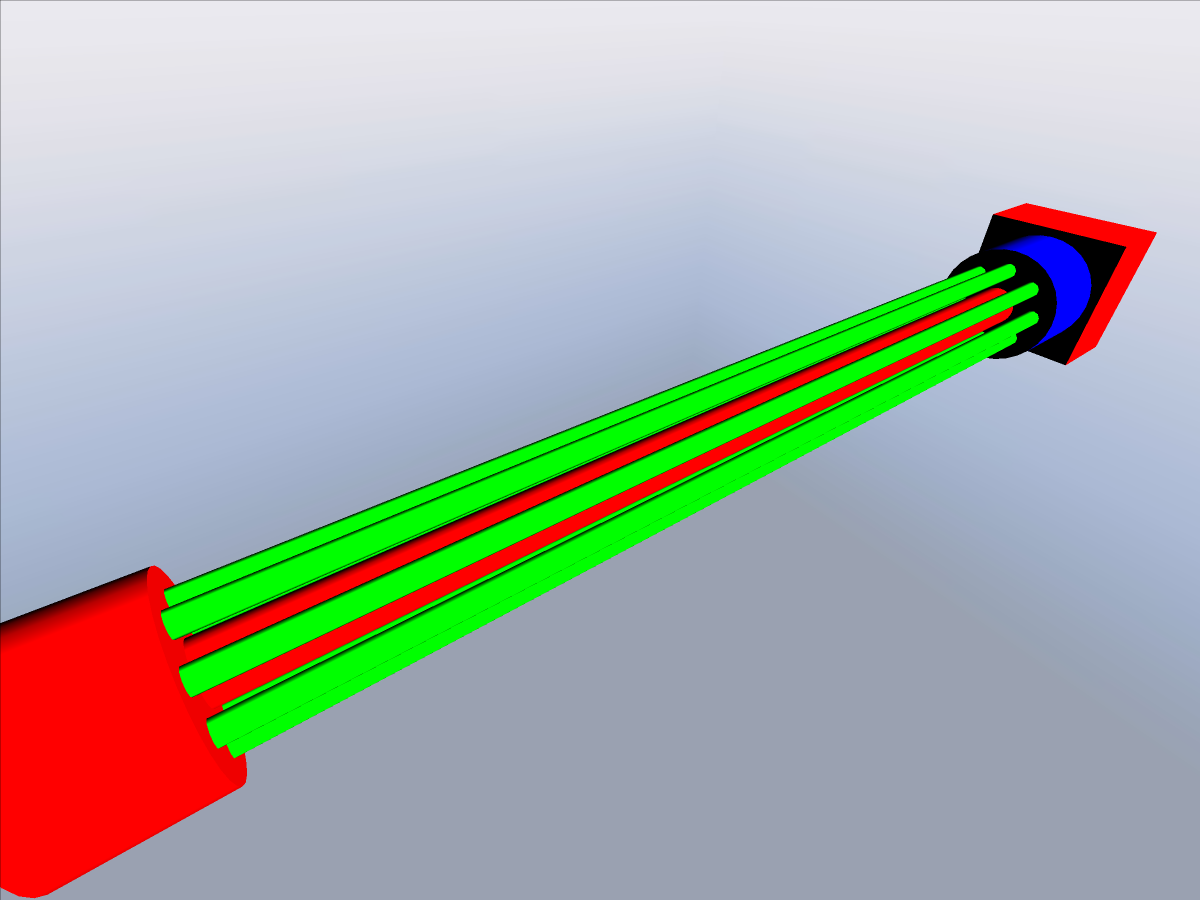
\includegraphics[width=\textwidth]{benchmark_contact/NSC001deg000}
        \caption{{\small Rotation: \SI{0}{\degree}}}    
        % \label{}
    \end{subfigure}
    \hfill
    \begin{subfigure}[b]{0.475\textwidth}  
        \centering 
        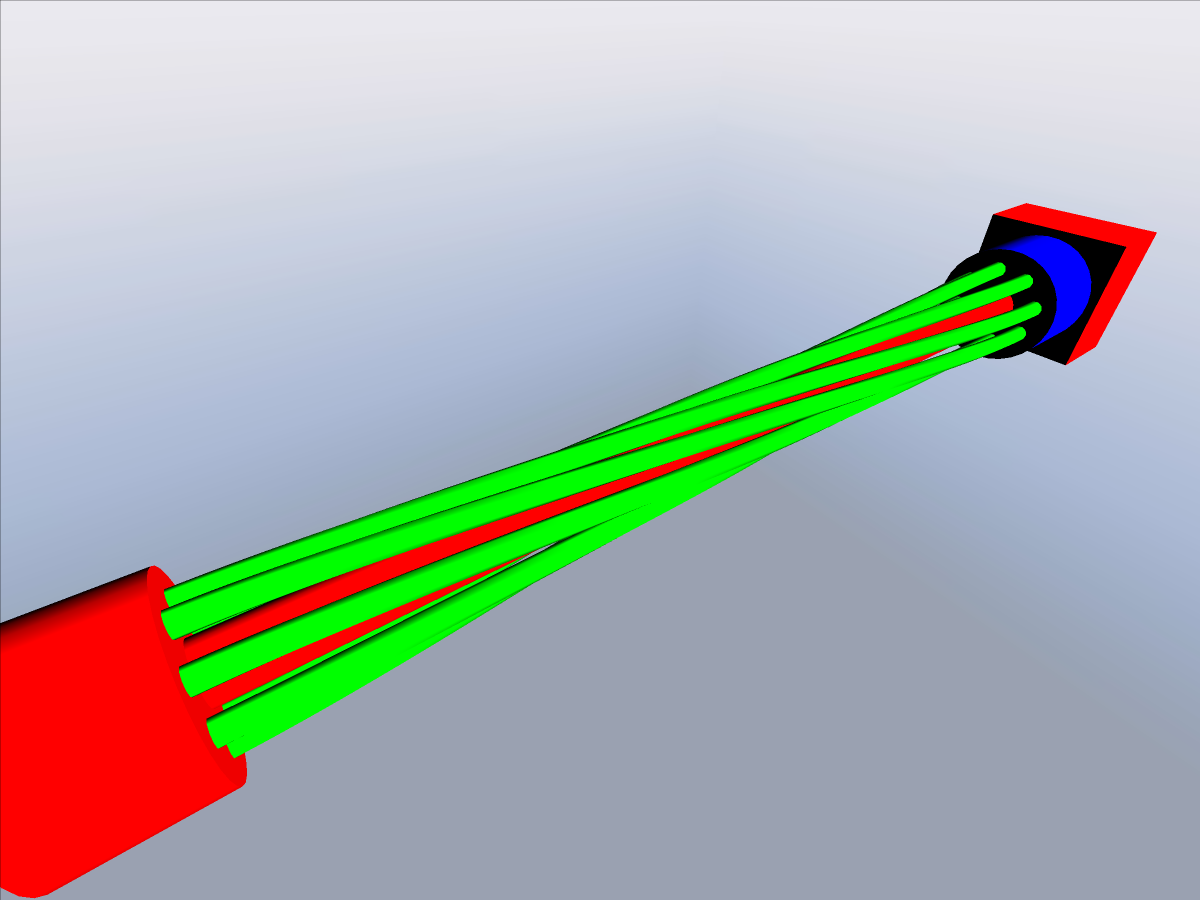
\includegraphics[width=\textwidth]{benchmark_contact/NSC001deg120}
        \caption[]{{\small Rotation: \SI{120}{\degree}}}    
        % \label{}
    \end{subfigure}
    \vskip\baselineskip
    \begin{subfigure}[b]{0.475\textwidth}   
        \centering 
        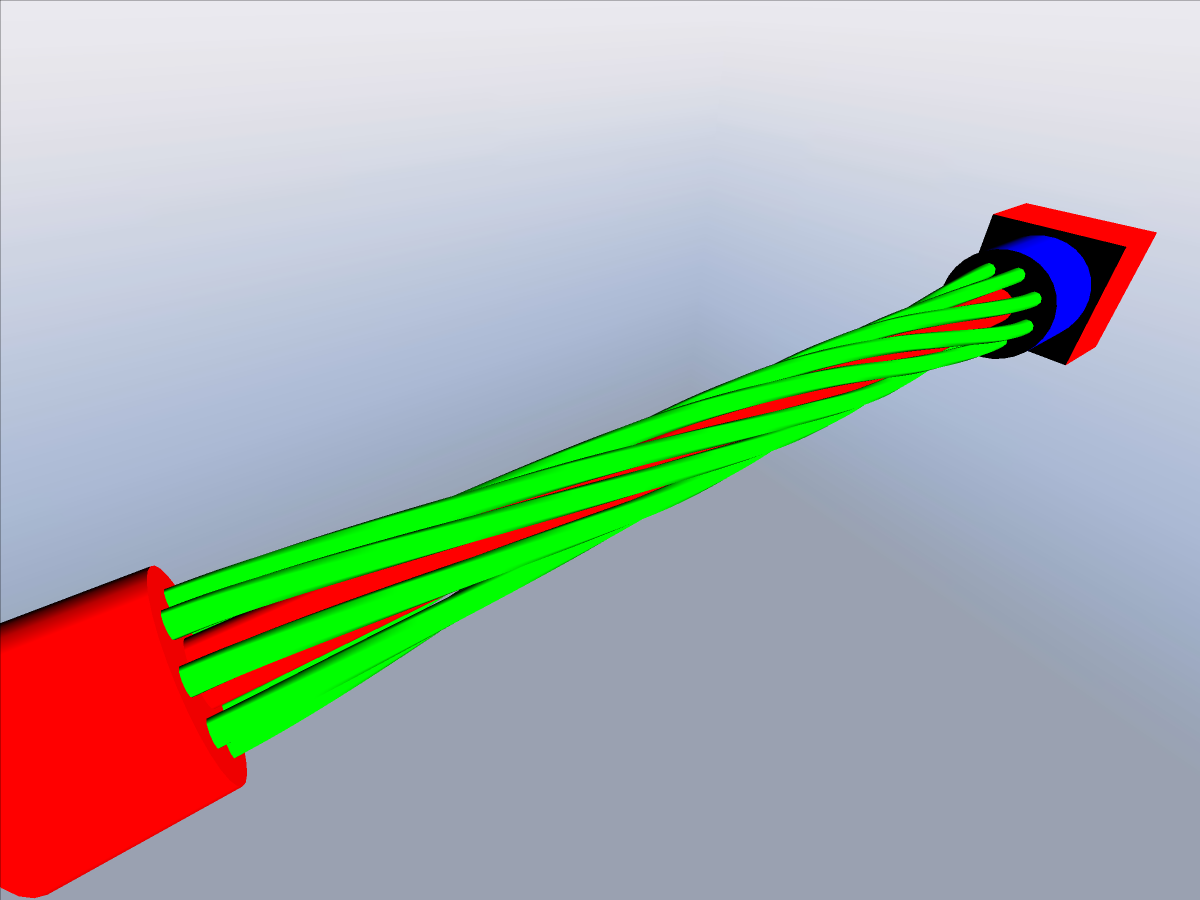
\includegraphics[width=\textwidth]{benchmark_contact/NSC001deg240}
        \caption[]{{\small Rotation: \SI{240}{\degree}}}    
        % \label{}
    \end{subfigure}
    \quad
    \begin{subfigure}[b]{0.475\textwidth}   
        \centering 
        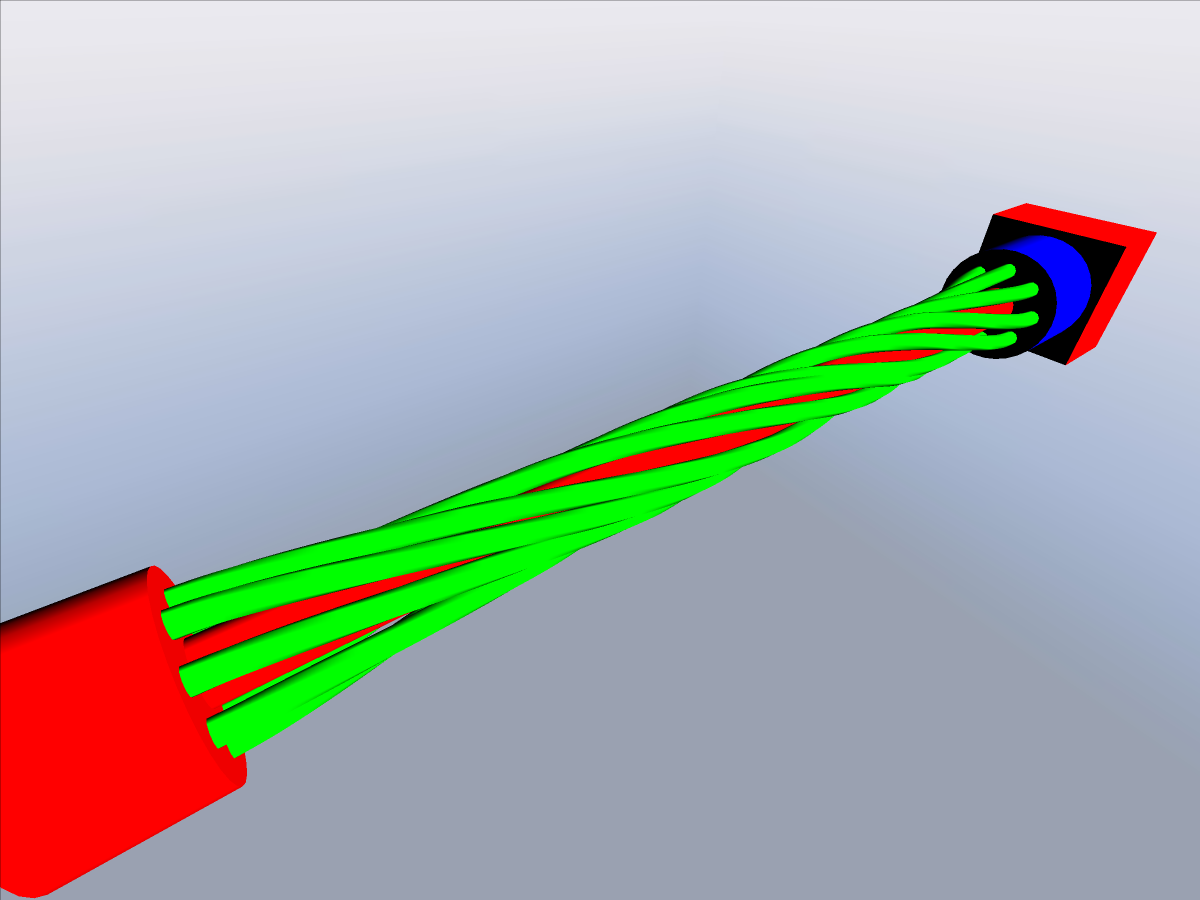
\includegraphics[width=\textwidth]{benchmark_contact/NSC001deg360}
        \caption[]{{\small Rotation: \SI{360}{\degree}}}    
        % \label{}
    \end{subfigure}
    \caption[Contact with rigid body]
    {\small Contact with rigid body (in red, elements that are fixed; in blue, the rotating shaft; in green, the IGA beams).} 
    \label{fig:contact}
\end{figure}

The dynamical analysis has been performed using the DVI time stepper \eqref{eq:dvi}-\eqref{eq:complementarity}. For this non-smooth dynamics problem, frictional contacts are enforced as complementarity constraints that do not require any tuning of penalty. %and the tangency of the contacting surfaces is guaranteed up to micrometric tolerances at each run of the SO-CCP solver. 
Note that when using conventional implicit or explicit integrators for smooth dynamics, high penalty stiffness would be needed to approximate contact between rigid materials without contact compenetration, but in turn this requires very short time steps to avoid numerical instability.

Multiple tests have been run with increasing time steps, from~\SI{1}{\ms} up to~\SI{75}{\ms}. 
This range includes values that are unusually large for this type of analysis; just for reference we report that we ran the same benchmark using the HHT time stepper and penalty contacts, but to avoid divergence the time step could not be larger than $h=\SI{1e-5}{\s}$.

The forces induced by beams on the shafts have been reported in~Fig.\ref{fig:contact_conv} and the relative error respect to a reference solution (computed with much shorter time step) is shown: being always under~\num{3}\% even for the largest time step is a good proof for the robustness of the DVI solver. It is remarkable that the solver was stable even for time steps larger than~\SI{100}{\ms}, but at that point the precision started to be compromised by other factors such as the precision of the collision detection algorithms etc. 

\begin{figure}[ht]
    \centering
    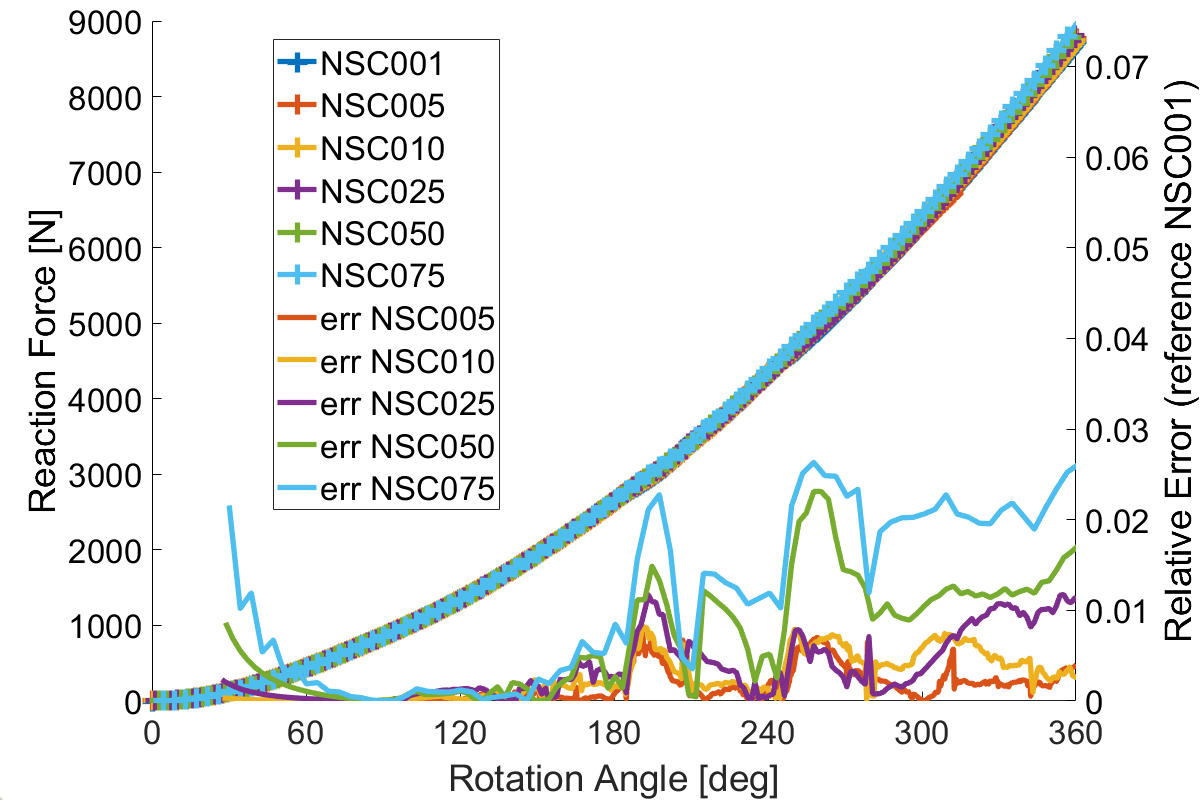
\includegraphics[width=0.7\textwidth]{benchmark_contact/ContactConvWithoutNSC100.png}
    \caption{Reaction force on the shaft for different time steps. In the legend, labels like NSC010 means Non-Smooth Contact test with time step $h=$\SI{10}{\ms} }
    \label{fig:contact_conv}
\end{figure}

%The overall trend of the root-mean-square error at increasing time step values is shown in~Fig.\ref{fig:contact_rmse}.

%\begin{figure}[ht]
%    \centering
%    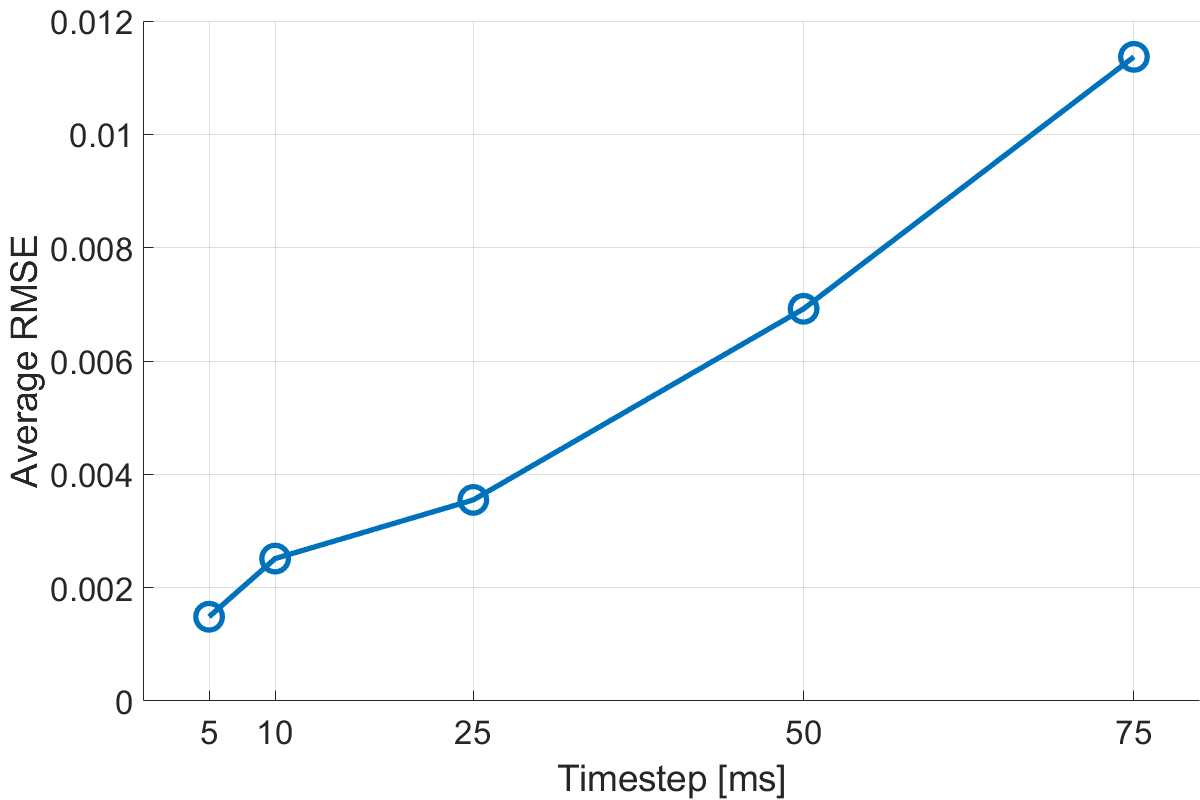
\includegraphics[width=0.8\textwidth]{benchmark_contact/contact_rmse.png}
%    \caption{RMSE of reaction forces on the shaft for different time steps.}
%    \label{fig:contact_rmse}
%\end{figure}

\subsection{Woven mesh}
In order to assess the performance of the DVI method for the case of mutual contact between IGA beams, a woven mesh of IGA beams has been reproduced and compared to literature~\cite{weeger2018frictional}.
The experiment consists in a 7x7 mesh where wires are clamped at one end, free at the other. Each wire is modeled with 64 nodes and a third-order IGA rod with cross-sectional radius of \SI{1}{mm}, Young modulus $E = \num{10e8}$ and Poisson ratio of $\nu = \num{0.5}$, for a total length $L = 4L_w = \SI{0.12}{m}$ where $L_w = \SI{0.03}{m}$ is the wavelength of the curve used to weave the mesh. Because of the non-smooth contact model no additional compliance parameter is required.

A distributed load of \SI{0.1}{N/m} is gradually applied to the beams in the vertical direction, and the DVI method is used to perform a non-linear analysis with a time step of~\SI{10}{ms} using the Interior-Point solver described in the previous example. Results are shown in~Fig.\ref{fig:woven_mesh}. % to reproduce the cited experiment. % but with significant difference that no progressive step has to be made. 
We remark that the time step could be increased up to~\SI{50}{ms} without incurring in divergence. Although the tolerance of the solver has been kept at the very strict threshold of~\num{1d-10} on residuals and complementarity, the computational time never exceeded \SI{0.997}{s/step} on a \SI{2.4}{GHz} Intel i7-4700 processor. %, with the perspective of achieving even faster performance if lower tolerances can be accepted and if future optimizations will be implemented in the code. %Contact points are computed automatically by the collision engine considering a sweep of spheres along the beams.

\begin{figure}[ht]
    \centering
    \begin{subfigure}[b]{0.475\textwidth}
        \centering
        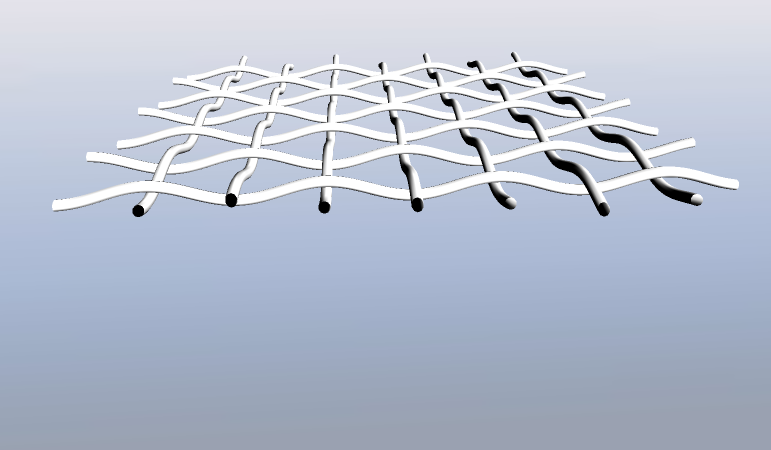
\includegraphics[width=\textwidth]{benchmark_mesh/mesh_load000.png}
        \caption{{\small Load: 0\%}}    
        % \label{}
    \end{subfigure}
    \hfill
    \begin{subfigure}[b]{0.475\textwidth}  
        \centering 
        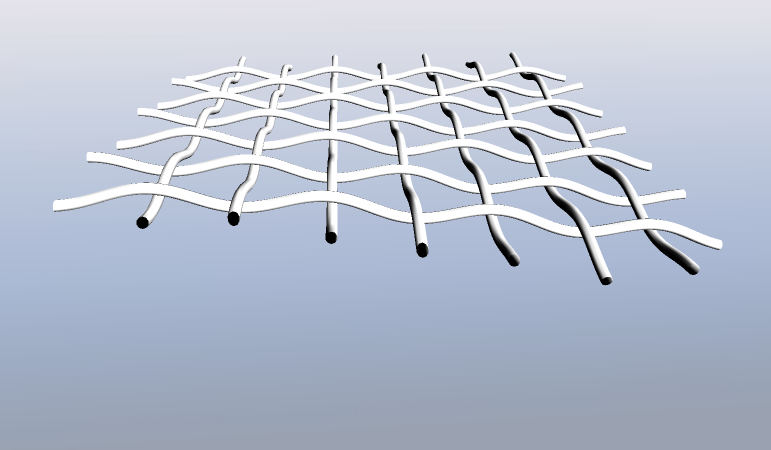
\includegraphics[width=\textwidth]{benchmark_mesh/mesh_load030.png}
        \caption{{\small Load: 30\%}}
        % \label{}
    \end{subfigure}
    \vskip\baselineskip
    \begin{subfigure}[b]{0.475\textwidth}   
        \centering 
        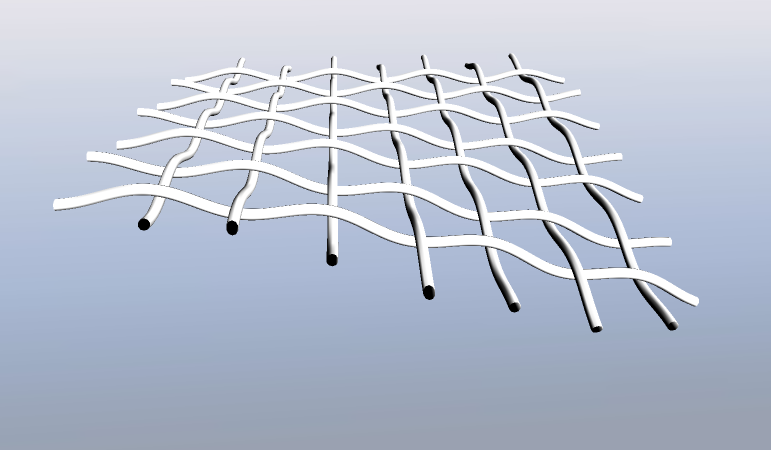
\includegraphics[width=\textwidth]{benchmark_mesh/mesh_load060.png}
        \caption{{\small Load: 60\%}}
        % \label{}
    \end{subfigure}
    \quad
    \begin{subfigure}[b]{0.475\textwidth}   
        \centering 
        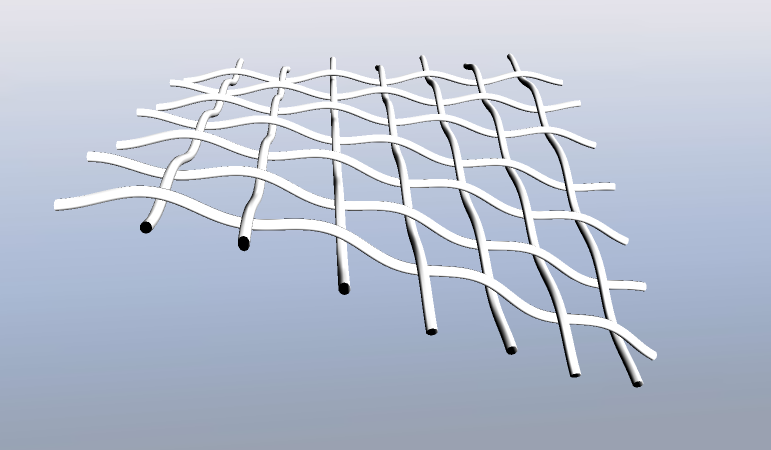
\includegraphics[width=\textwidth]{benchmark_mesh/mesh_load100.png}
        \caption{{\small Load: 100\%}}
        % \label{}
    \end{subfigure}
    \caption[Woven mesh]
    {\small Snapshots from the simulation of the woven mesh, for increasing load.} 
    \label{fig:woven_mesh}
\end{figure}


\section{Conclusions}

A geometrically-exact spatial Cosserat rod has been implemented via IGA discretization, using quaternions as rotational coordinates. We implemented the model in a open-source physics library using C++ language and we tested it in various non-linear static and dynamic problems, showing generality, robustness and efficiency of the formulation. 

Using a DVI time stepping scheme and a SO-CCP solver, we proved that simulations with non-smooth frictional contacts between IGA beams and moving shapes can be performed with large time steps. The enhanced robustness and stability indicate that the DVI method is a viable alternative to conventional methods based on contact penalty. 


%
% ---- Bibliography ----
%
\section*{\refname}
\bibliographystyle{plain}
\bibliography{mybib,BibMBS,BibFEM}


\appendix
\section{Constitutive models for beams}
\label{sec:constitutive}

In the most generic case, \eqref{eq:mnconstitutive} may be a non-linear function, but in the following we present special cases of practical interest.

\subsection{Generic linear elasticity}
\label{sec:generic}

The generic case of constitutive model for the Cosserat rod, with linear elasticity, requires a matrix $\amatr{E} \in \mathbb{R}^{6x6}$, not necessarily sparse. Such matrix can be provided by some detailed 3D FEA analysis of a chunk of beam, in a preprocessing stage.
%
\begin{align}
    \left\{  
    \begin{array}{c}
     \avect{n} \\
     \avect{m} 
    \end{array}
    \right\}
    &= 
    \amatr{E}
    \left\{  
    \begin{array}{c}
     \avect{\epsilon} \\
     \avect{\kappa}
    \end{array}
    \right\}
\end{align}

We remark that, depending on the 36 values used in the 6x6 $\amatr{E}$ matrix,  $\avect{n}$ and $\avect{m}$ might have coupled effects. Figure \ref{fig:section} shows the reference coordinate system of the section.

\begin{figure}[ht]
    \centering
    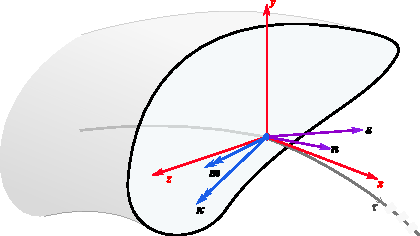
\includegraphics[width=0.60\textwidth]{section_beam.pdf}
    \caption{Section of the beam. Generic case.}
    \label{fig:section}
\end{figure}


\subsection{Basic diagonal linear elasticity}
\label{sec:basic}

For centered symmetric sections, the previous relation can be simplified. In fact one can express the constitutive relation via a linear mapping where $\avect{n}$ and  $\avect{m}$ effects are uncoupled:
%
\begin{align}
\avect{n} &= \avect{n}(\avect{\epsilon}) \\ 
\avect{m} &= \avect{m}(\avect{\kappa})
\label{eq:mn}
\end{align}
%
In detail, with linear elasticity, a very common case is the linear mapping:
%
\begin{align}
\avect{n} &= \amatr{C} \avect{\epsilon}  \\ 
\avect{m} &= \amatr{D} \avect{\kappa} 
\label{eq:mnlin}
\end{align}
%
where one simply uses the material matrices:
%
\begin{align}
	\amatr{C} = 
	\left[  
	\begin{array}{ccc}
	 E A & 0 & 0 \\
	 0 & G A k_y & 0 \\
	 0 & 0 & G A k_z 
	\end{array}
	\right]
	\quad
	\amatr{D} = 
	\left[  
	\begin{array}{ccc}
	 G J & 0 & 0 \\
	 0 & E I_y & 0 \\
	 0 & 0 & E I_z
	\end{array}
	\right]
\end{align}
%
for given material Young' modulus $E$, shear modulus $G$, area $A$, Timoshenko shear correction factors $k_y,k_z$, torsion constant $J$, and second moments of area $I_y, I_z$ computed in the section reference. Note that the center of axial forces $C_a$ and the shear center $C_s$ are in the origin, by assumption. See Fig.~\ref{fig:section_diagonal}.

\begin{figure}[ht]
    \centering
    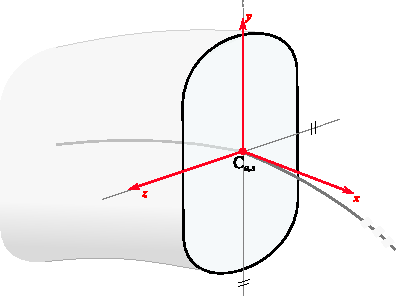
\includegraphics[width=0.60\textwidth]{section_beam_diagonal.pdf}
    \caption{Section of the beam. Simplified case (diagonal $\amatr{E}$).}
    \label{fig:section_diagonal}
\end{figure}


\subsection{Advanced section for linear elasticity}
\label{sec:advanced}

A more general constitutive model is the one depicted in Fig.~\ref{fig:section_advanced}, where the $I_y, I_z$ are computed respect to an auxiliary reference $C_a$, center of axial forces, that has displacement $y_a, z_a$ and rotation $\alpha$ respect to the reference center line of the beam~\cite{MASARATI-2014-IJSS} .

Also, in case of non-symmetric sections, it may happen that the shear center $C_s$ does not coincide with $C_a$; if so, one can provide displacements $y_s, z_s$ and rotation $\beta$ of the reference of the shear center $C_s$ respect to the reference center line of the beam. 

Usually, for symmetric sections, it tends to $y_s=y_a$, $z_s=z_a$, $\alpha=\beta$. For simple problems like rectangular or circular sections centered on the reference line of the beam, one has $y_s=y_a=0$, $z_s=z_a=0$, $\alpha=\beta=0$.

\begin{figure}[ht]
    \centering
    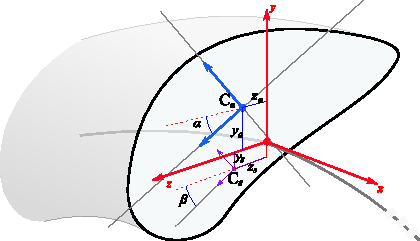
\includegraphics[width=0.60\textwidth]{section_beam_advanced.pdf}
    \caption{Section of the beam. Advanced case.}
    \label{fig:section_advanced}
\end{figure}

The linear model becomes:
%
\begin{align}
\left\{  
	\begin{array}{c}
	 \avect{n} \\
	 \avect{m} 
	\end{array}
	\right\}
	&= 
	\left[  
	\begin{array}{cccccc}
	 a_{11} & 0 & 0 & 0 & a_{12} & a_{13} \\
	 0      & s_{11} & s_{12} & s_{13} & 0 & 0 \\
	 0      & s_{21} & s_{22} & s_{23} & 0 & 0 \\
	 0      & s_{31} & s_{32} & s_{33} & 0 & 0 \\
	 a_{21} & 0      & 0      & 0      & a_{22} & a_{23} \\
	 a_{31} & 0      & 0      & 0      & a_{32} & a_{33}
	\end{array}
	\right]
	\left\{  
	\begin{array}{c}
	 \avect{\epsilon} \\
	 \avect{\kappa}
	\end{array}
	\right\}
\end{align}

Here the components $a_{ij}=\amatr{A}$ and $s_{ij}=\amatr{S}$ are obtained by rotations $\amatr{R}$ and translations $\amatr{T}$ of the diagonal constitutive matrices $\amatr{A}_{C_a}$ and $\amatr{S}_{C_s}$:
%
\begin{align}
\amatr{A} &= \amatr{T}_{C_a} \amatr{R}_{C_a} \amatr{A}_{C_a}  \amatr{R}_{C_a}^T \amatr{T}_{C_a}^T \\
\amatr{S} &= \amatr{R}_{C_s}^T \amatr{T}_{C_s}^{-1} \amatr{S}_{C_s}  \amatr{T}_{C_s}^{-T} \amatr{R}_{C_s}
\end{align}
%
where
% 
\begin{align}
\amatr{A}_{C_a} = 
	\left[  
	\begin{array}{ccc}
	 E A & 0 & 0 \\
	 0 & E I_y & 0 \\
	 0 & 0 & E I_z 
	\end{array}
	\right]
	\quad
	\amatr{S}_{C_s} = 
	\left[  
	\begin{array}{ccc}
	 G A k_y  & 0 & 0 \\
	 0 & G A k_z & 0 \\
	 0 & 0 & G J
	\end{array}
	\right]
\end{align}
	
The above model requires the following parameters: Young modulus $E$, shear modulus $G$, area $A$, Timoshenko shear correction factors $k_y,k_z$, torsion constant $J$, and second moments of area $I_y, I_z$, as the diagonal simplified model, plus the  position and rotation of $C_a$ as $y_a, z_a$ and $\alpha$, plus the position and rotation of $C_s$ as $y_s, z_s$ and $\beta$.

% REMOVED SUBSECTION ON MESH-INTEGRATED SECTION, 
% IT SEEMS TO MUCH. REMOVE COMMENT IN FRONT
% OF \input{...} TO ENABLE IF NEEDED. ALESSANDRO.
%\input{"chapter_integrated_section.tex"}

%\subsection{Other}
%
%For the case of elasto-plastic constitutive models, see %later.

% REMOVED SUBSECTION ON BEAM PLASTICITY, 
% IT SEEMS TO MUCH. REMOVE COMMENT IN FRONT
% OF \input{...} TO ENABLE IF NEEDED. ALESSANDRO.
%\input{"chapter_plasticity.tex"}




\end{document}
